% ============================================================
%  ECHORA — UON Group Project Report (ENG4006, AS2)
%  University of Northampton submission (7500-word group report)
%
%  Formatting follows "Guidelines on the Format of the Final Report":
%   - English, Times New Roman 12pt body, 1.5 line spacing, justified
%   - Chapter headings 14pt bold; section 12pt bold; subsection 12pt bold italic
%   - Each chapter begins on a new page, preceded by the word "Chapter" + number
%   - Arabic numeral numbering (1, 1.1, 1.1.1)
%   - Preliminaries: Title, Abstract, Acknowledgements, Contents,
%     Lists of Tables and Figures, Glossary
%   - End matter: References (Harvard), Appendices
%
%  Build with pdflatex (run twice for the table of contents / lists):
%     pdflatex main
%     pdflatex main
% ============================================================
\documentclass[12pt,a4paper]{report}

% ----------------------------
% Page layout
% ----------------------------
\usepackage[a4paper,margin=1in]{geometry}

% ----------------------------
% Fonts — Times New Roman look (Times-compatible) + T1 encoding
% ----------------------------
\usepackage[T1]{fontenc}
\usepackage[utf8]{inputenc}
\usepackage{newtxtext}   % Times New Roman-like serif for the text
\usepackage{newtxmath}   % matching maths

% ----------------------------
% Line spacing 1.5, justified body with first-line indent
% ----------------------------
\usepackage{setspace}
\onehalfspacing
\setlength{\parindent}{0.5cm}
\setlength{\parskip}{4pt plus 1pt}

% ----------------------------
% Figures, tables, colour
% ----------------------------
\usepackage{graphicx}
\graphicspath{{images/}}
\usepackage{float}
\usepackage{array}
\usepackage{longtable}
\usepackage{booktabs}
\usepackage[table]{xcolor}
\usepackage{caption}
% Captions (title and source) are set smaller than the 12pt body text.
% Tables: title above, source below.  Figures: title and source both below.
\captionsetup{font=small,labelfont=bf,justification=centering}
\captionsetup[table]{position=top,skip=6pt}
\captionsetup[figure]{position=bottom,skip=6pt}

% Source line placed at the foot of a table or figure.
\newcommand{\source}[1]{\par\vspace{4pt}{\small\itshape Source: #1}}

% ----------------------------
% Headings: Chapter 14pt bold, Section 12pt bold, Subsection 12pt bold italic
% Chapters start on a new page and are labelled "Chapter N".
% ----------------------------
\usepackage{titlesec}
\titleformat{\chapter}[display]
  {\normalfont\bfseries\fontsize{14}{18}\selectfont}
  {\chaptertitlename\ \thechapter}{6pt}
  {\fontsize{14}{18}\selectfont}
\titlespacing*{\chapter}{0pt}{0pt}{16pt}
\titleformat{\section}
  {\normalfont\bfseries\fontsize{12}{15}\selectfont}{\thesection}{0.6em}{}
\titleformat{\subsection}
  {\normalfont\bfseries\itshape\fontsize{12}{15}\selectfont}{\thesubsection}{0.6em}{}
\titleformat{\subsubsection}
  {\normalfont\itshape\fontsize{12}{15}\selectfont}{\thesubsubsection}{0.6em}{}

% ----------------------------
% Page numbers (bottom-centre), no rules
% ----------------------------
\usepackage{fancyhdr}
\pagestyle{fancy}
\fancyhf{}
\fancyfoot[C]{\thepage}
\renewcommand{\headrulewidth}{0pt}
\renewcommand{\footrulewidth}{0pt}
\fancypagestyle{plain}{\fancyhf{}\fancyfoot[C]{\thepage}\renewcommand{\headrulewidth}{0pt}}

% ----------------------------
% Hyperlinks (plain, no coloured boxes)
% ----------------------------
\usepackage[hidelinks]{hyperref}

% ----------------------------
% For inserting the official UON assignment cover sheet as page 1.
% cover_sheet.pdf is exported from "ASSIGNMENT  COVER  SHEET.docx";
% re-export it after editing the Word form.
% ----------------------------
\usepackage{pdfpages}

% Convenience: a Harvard reference entry with a hanging indent.
\newcommand{\refent}[1]{\par\hangindent=1.27cm\hangafter=1 #1\par\medskip}

\begin{document}

% ============================================================
%  PRELIMINARIES  (roman page numbers, not counted in the word limit)
% ============================================================
\pagenumbering{roman}

% ---- Official UON assignment cover sheet (unnumbered, first page) ----
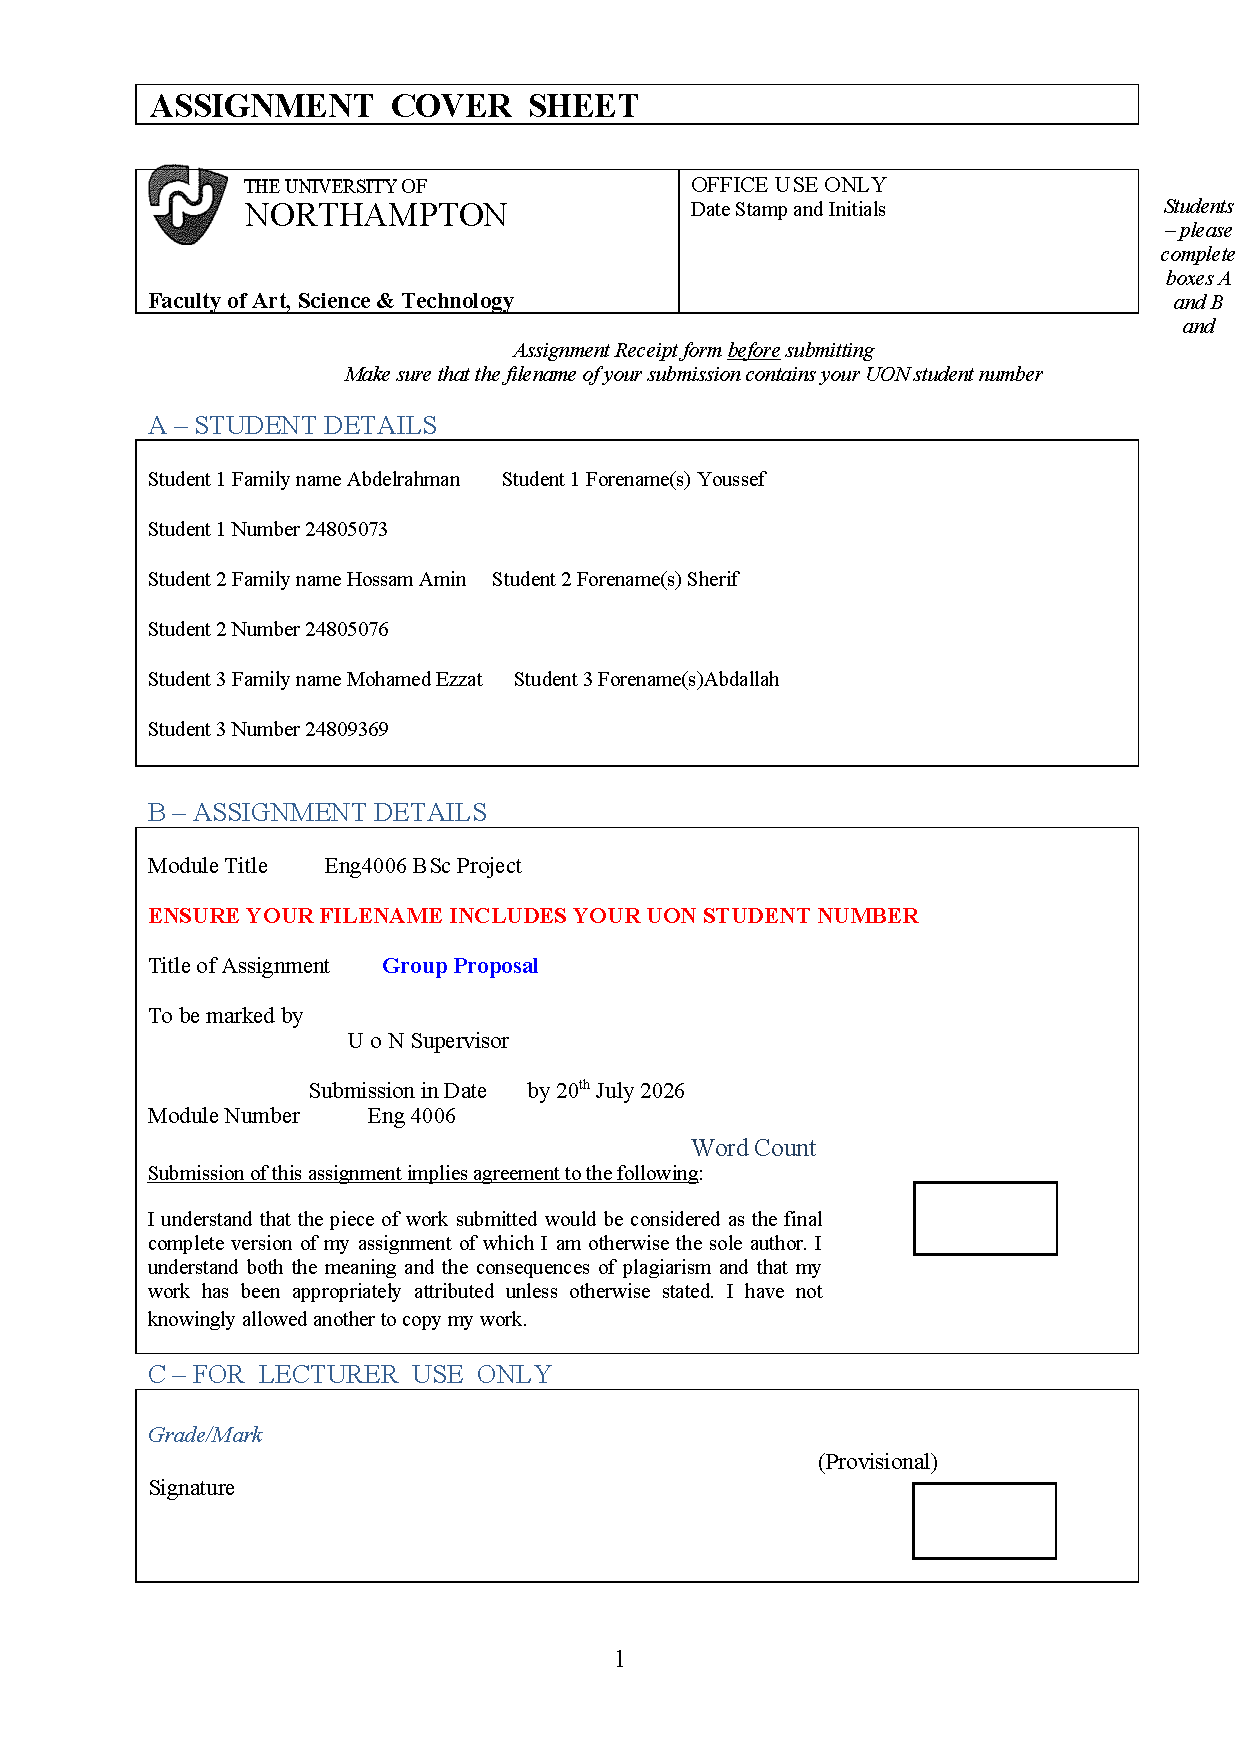
\includepdf[pages=-]{cover_sheet.pdf}

% ---- Title page ----
% ------------------------------------------------------------
%  Title page — laid out in the style of the standard UON
%  dissertation cover sheet (see cover.jpeg): centred UON mark,
%  faculty, title, author block, supervisor, date, and the
%  formal submission statement. Partner marks (AASTMT) and the
%  project mark (ECHORA) sit in a footer row.
% ------------------------------------------------------------
\begin{titlepage}
\thispagestyle{empty}
\centering
\setstretch{1.15}

\vspace*{0.2cm}

% ---- University mark ----

\includegraphics[width=0.34\textwidth]{uon_logo.png}

\vspace{0.7cm}

Faculty of Arts, Science and Technology

\vspace{0.8cm}

% ---- Title ----
{\bfseries ECHORA --- ``An AI-Powered Sensory Substitution System\\
for Blind and Low-Vision Users''.\par}

\vspace{0.7cm}

By

\vspace{0.7cm}

{\bfseries Yossef Ashraf \quad Sherif Amin \quad Abdallah Ezzat}

\vspace{0.7cm}

ENG4006 Group Industry Project --- Final Report (AS2)

\vspace{0.8cm}

{\bfseries Supervisor: Alaa Hassan\par}

\vspace{0.8cm}

July 2026

\vspace{0.9cm}

{\bfseries Submitted to The University of Northampton\par}
{\bfseries in partial fulfilment of the requirements for the degree of\par}
{\bfseries BSc Computer Scienc\par}

\vspace{0.5cm}

in collaboration with the\\
Arab Academy for Science, Technology \& Maritime Transport (AASTMT)

\vfill

% ---- Partner and project marks ----
\begin{minipage}{0.45\textwidth}
  \centering
  
\includegraphics[height=2.0cm]{aast_logo.png}
\end{minipage}%
\begin{minipage}{0.45\textwidth}
  \centering
  
\includegraphics[height=1.2cm]{logo.png}
\end{minipage}

\vspace{0.2cm}

\end{titlepage}
\clearpage


% ---- Abstract ----
\chapter*{Abstract}
\addcontentsline{toc}{chapter}{Abstract}

Blind and low-vision (BLV) people face daily difficulty in reading text, recognising objects, and moving safely through the spaces around them. Most assistive tools available today solve only one of these problems at a time. A smart cane warns about nearby obstacles but cannot read a sign; a reading device speaks printed text but gives no sense of the space ahead. This leaves users switching between several single-purpose devices and still missing an integrated picture of their surroundings.

This report presents Echora, a wearable assistive system that brings several of these functions together in one adaptive framework. Echora pairs a head-worn depth camera with a wrist-worn haptic (vibration) module and runs its artificial-intelligence models locally on a connected computer, so no internet connection or cloud service is required. The system operates in five modes: navigation (obstacle awareness with distance zones), text reading, face recognition, Egyptian banknote identification, and hand-guidance for reaching objects. A safety-first state machine chooses the right mode automatically from what the camera sees and how the user is moving, and it always falls back to navigation when a close obstacle appears.

The prototype was built as real hardware, consisting of a 3D-printed headset and a custom-designed haptic circuit board, and was evaluated both at the model level and as a complete system. The custom Egyptian banknote detector reached a mean Average Precision (mAP@0.5) of 0.991 across eleven denominations, and the accessibility detector for doors, handles, and lift controls reached 0.726. The full pipeline ran in real time at roughly 20 frames per second, and every automated integration test and system-level scenario passed, including the critical safety rule that a danger-zone obstacle always forces a return to navigation. These results show that a unified, privacy-preserving, real-time assistive system can be delivered on ordinary computing hardware. The report closes with a critical review of the outcomes and a set of clear directions for future work.

\vspace{0.8cm}
\noindent\textbf{Keywords:} assistive technology, sensory substitution, computer vision, depth sensing, haptic feedback, blind and low-vision, real-time systems.

\clearpage


% ---- Acknowledgements ----
\chapter*{Acknowledgements}
\addcontentsline{toc}{chapter}{Acknowledgements}

We would like to thank our supervisors and tutors at the University of Northampton and at the Arab Academy for Science, Technology \& Maritime Transport for their guidance, feedback, and encouragement throughout this project. Their advice on both the technical direction and the written work was invaluable.

We are also grateful to the members of the blind and low-vision community whose experiences and feedback shaped the goals of this project and kept our design focused on real, everyday needs. Finally, we thank our families and friends for their patience and support during the long hours of building, testing, and writing.

\clearpage


% ---- Declaration on the use of generative AI (UON policy) ----
\chapter*{Declaration on the Use of Generative Artificial Intelligence}
\addcontentsline{toc}{chapter}{Declaration on the Use of Generative Artificial Intelligence}

In line with the University of Northampton's policy on the use of generative
artificial intelligence, we declare the following.

All of the work described in this report is our own. The system design, the
software, the datasets, the model training, the experiments, and the results
reported here were produced entirely by the project team. Every chapter of this
report was first written by us as a full draft in our own words, based on our own
work and our own reading.

After that first draft was complete, we used a generative AI assistant as a
language tool only. We used it to check spelling, to correct grammar and
punctuation, to improve the clarity and flow of sentences that we had already
written, and to check that the document followed the required formatting and
structure. In every case we reviewed the suggestions ourselves, accepted only
those we agreed with, and kept final control of the wording.

We did not use AI to generate the ideas, arguments, technical content, results,
or conclusions of this report, and we did not use it to produce or suggest any
reference. All sources cited were found, read, and verified by us. We understand
that information produced by AI can be inaccurate or biased, and we have
therefore checked all remaining content against our own work and sources.

Full details of how the tool was used are given in Appendix~D.

\clearpage


% ---- Table of Contents ----
\clearpage
\tableofcontents

% ---- Lists of Tables and Figures ----
\clearpage
\listoftables
\clearpage
\listoffigures

% ---- Glossary ----
\clearpage
\chapter*{Glossary of Acronyms}
\addcontentsline{toc}{chapter}{Glossary of Acronyms}

\begin{longtable}{p{0.20\textwidth} p{0.74\textwidth}}
\toprule
\textbf{Acronym} & \textbf{Expansion} \\
\midrule
\endfirsthead
\toprule
\textbf{Acronym} & \textbf{Expansion} \\
\midrule
\endhead
AASTMT & Arab Academy for Science, Technology \& Maritime Transport \\
AI & Artificial Intelligence \\
BLV & Blind and Low-Vision \\
CPU & Central Processing Unit \\
FPS & Frames Per Second \\
GPU & Graphics Processing Unit \\
IMU & Inertial Measurement Unit \\
IoU & Intersection over Union \\
mAP & mean Average Precision \\
OCR & Optical Character Recognition \\
RGB-D & Red, Green, Blue and Depth \\
SDG & Sustainable Development Goal \\
TTS & Text-to-Speech \\
UON & University of Northampton \\
YOLO & You Only Look Once \\
\bottomrule
\end{longtable}
\clearpage


% ============================================================
%  BODY  (arabic page numbers; word count starts here)
% ============================================================
\clearpage
\pagenumbering{arabic}

\chapter{Introduction}
\label{ch:intro}

\section{Background and Rationale}

Sight does a great deal of quiet work in daily life. It lets us read a sign, find a door handle, recognise a friend, check the value of a banknote, and step around a chair without thinking about any of it. For blind and low-vision (BLV) people, each of these small tasks can become slow, uncertain, or unsafe. Traditional aids such as the white cane and the guide dog are genuinely valuable, but they mainly help with obstacles close to the body and give very little information about \emph{what} an object is, what a sign says, or who is standing nearby.

Over the last few years, advances in artificial intelligence (AI), depth cameras, and small wearable electronics have opened a new path. Instead of restoring sight, these technologies can \emph{substitute} for it, taking visual information and delivering it through hearing and touch. This idea, known as sensory substitution, is the foundation of this project. The problem it addresses is not a shortage of clever gadgets; it is that most existing products each solve a single task. One device reads text, another warns about obstacles, a third recognises faces. A user who wants all of these must carry several devices and still lacks a joined-up understanding of the scene in front of them.

The need is also large. Vision impairment affects hundreds of millions of people worldwide, the numbers are rising with ageing populations, and the effect on independence, employment, and confidence is significant. This makes a strong case for an assistive system that is affordable, works without an internet connection, and brings several everyday functions together rather than treating each one separately.

\section{Motivation and Impact}

The motivation for Echora is grounded in both the scale of vision loss and the limits of what is currently available. Globally, billions of people live with some form of eye condition, and a large share of these lead to moderate or severe vision impairment. The picture is similar in the Middle East and in Egypt specifically, where the blind and low-vision population is substantial and, worryingly, the trend in sight loss is rising rather than falling over time. This growth places pressure not only on individuals and families but on healthcare and support systems as a whole.

The impact is not only personal but economic. Reduced vision lowers workforce participation and efficiency and increases dependency, which together create considerable annual productivity losses. Solutions that restore even part of a person's independence therefore carry a social and economic value well beyond the individual user. Echora is motivated by exactly this: rather than adding one more single-purpose gadget to an already fragmented market, it aims to give users a broader, more proactive understanding of their surroundings while keeping the cost low by performing the heavy computation on an ordinary computer. In doing so, the project also supports several United Nations Sustainable Development Goals, notably good health and well-being (SDG~3), industry and innovation (SDG~9), reduced inequalities (SDG~10), and inclusive, accessible communities (SDG~11).

\section{Project Aims and Objectives}

\subsection{Project Aim}

The aim of this project was to design, build, and evaluate \textbf{Echora}: a wearable, AI-powered sensory-substitution system that gives BLV users a richer, real-time sense of their surroundings through audio and haptic (vibration) feedback, while keeping all processing local for privacy and low latency.

\subsection{Project Objectives}

To meet that aim, the project set the following objectives:

\begin{itemize}
    \item Build a wearable sensing unit around a depth camera, together with a wrist-worn haptic module, and connect them to a computer that performs the AI processing.
    \item Provide continuous obstacle awareness that classifies nearby objects into clear danger, warning, and safe zones and communicates their direction.
    \item Add practical everyday functions: reading printed text aloud, recognising enrolled people, identifying Egyptian banknotes, and guiding the user's hand to reach an object.
    \item Combine these functions under a single context-aware controller that switches between them automatically and always gives priority to safety.
    \item Keep the whole pipeline running in real time on ordinary computing hardware, with no reliance on cloud services.
    \item Evaluate both the individual AI models and the complete integrated system against clear, measurable criteria.
\end{itemize}

\section{Scope}

The project delivers a working prototype rather than a finished commercial product. The five perception functions above are all implemented and tested. To keep the work achievable within the available time, some longer-term features were deliberately left for future development: a fully wireless link between the glasses and the computer (the prototype uses a wired depth camera), encryption of stored face data at rest, and semantic interpretation of traffic and warning signs. These are discussed honestly in the conclusions. Echora is designed to \emph{complement} the white cane and guide dog, not to replace them.

\section{Summary of Main Results}

The prototype was built as real, wearable hardware, consisting of a 3D-printed and hand-finished headset carrying the depth camera and a custom-designed circuit board driving a wrist array of vibration motors, and was then evaluated at two levels. At the model level, the custom Egyptian banknote detector achieved a mean Average Precision (mAP@0.5) of 0.991 across eleven denominations, and the accessibility detector for doors, handles, and lift controls reached 0.726. At the system level, the complete pipeline ran in real time at roughly 20 frames per second while detecting, tracking, and zoning multiple obstacles at once. Every automated integration test passed, and every system-level scenario behaved as expected, including the most important safety rule: a danger-zone obstacle always forced an immediate return to navigation mode, regardless of what the system was doing. Taken together, these results show that a unified, private, real-time assistive system is achievable on standard hardware.

\section{Report Structure}

The rest of this report is organised as follows. Chapter~\ref{ch:lit} reviews existing assistive products and the research that informed the design. Chapter~\ref{ch:dev} describes how the system was developed, covering the methodology, the architecture, the hardware build, and the datasets used to train the custom models. Chapter~\ref{ch:results} presents and critically reviews the results. Chapter~\ref{ch:conclusion} evaluates how well the project met its objectives and sets out recommendations for future work.

\chapter{Literature Review}
\label{ch:lit}

This chapter reviews the products and research that shaped Echora's design. It looks first at assistive tools already on the market, then at the academic work on sensory substitution, and finally draws out the gap that Echora sets out to fill. Throughout, the aim is not just to describe each system but to weigh its strengths and weaknesses against the needs of a BLV user who wants one integrated aid rather than several separate ones.

\section{Existing Assistive Products}

Commercial assistive technology for BLV users has grown quickly, but it remains fragmented. The clearest way to see this is to compare a few representative products.

\textbf{Camera-and-audio glasses.} Envision Glasses and Seleste are smart glasses that use a camera and AI to describe scenes and read text aloud. Their strengths are genuine: Envision in particular reads printed text very well and sits within a polished, well-supported product. However, both are essentially \emph{semantic} tools. They tell the user what text or objects are present, but they do not sense depth, so they cannot build a reliable picture of how far away things are or warn about an approaching obstacle. Neither offers any touch-based feedback, and neither helps the user physically reach or interact with an object. For continuous, moment-to-moment spatial awareness while walking, this is a real limitation (Envision, 2026a; Seleste, 2023).

\textbf{Wearable reading cameras.} OrCam MyEye is a small camera that clips onto ordinary glasses and speaks text and recognised faces. It is compact, fast, and easy to use, and its OCR quality is high. Its weakness is the same as the glasses above but sharper: it has no depth perception, no obstacle awareness, and no haptic channel. It is excellent at delivering short pieces of information on demand, but it offers little for safe movement or object interaction (OrCam Technologies, 2023).

\textbf{Obstacle-sensing mobility aids.} WeWalk and the Sunu Band approach the problem from the opposite direction. WeWalk adds ultrasonic sensing and vibration to a white cane, and Sunu is a wrist band that vibrates when objects are near. Both are portable, intuitive, and sit comfortably alongside familiar habits. Yet their sensing is limited to basic ``something is close'' proximity. They do not identify \emph{what} an object is, cannot read text or recognise people, and build no real model of the space. They improve safety but add no semantic understanding (WeWALK, 2026; Sunu, 2018).

The pattern is consistent: reading-and-recognition devices ignore space and touch, while mobility aids ignore meaning. A user who wants both must combine products that were never designed to work together. Table~\ref{tab:comparison}, adapted from the market analysis, sets these systems side by side against the integrated capability Echora targets.

Looking at the wider market through standard analytical lenses tells the same story. A SWOT view shows that the main \emph{opportunity} is precisely the integration gap, since no mainstream product combines depth-based navigation, reading, recognition, and touch feedback, while the main \emph{threats} are the strong brand presence of established devices and the cost of specialised hardware. A PESTEL view highlights favourable technological and social factors (cheaper AI compute, growing accessibility awareness) but also real regulatory and ethical pressure around cameras and biometric data. The clear conclusion for positioning is that Echora should not try to beat OrCam at reading or WeWalk at obstacle sensing on their own terms; its distinct value is in \emph{unifying} these functions affordably and privately, on hardware people may already own.

\begin{table}[H]
\centering
\caption{Comparison of existing assistive technologies against the proposed Echora system.}
\label{tab:comparison}
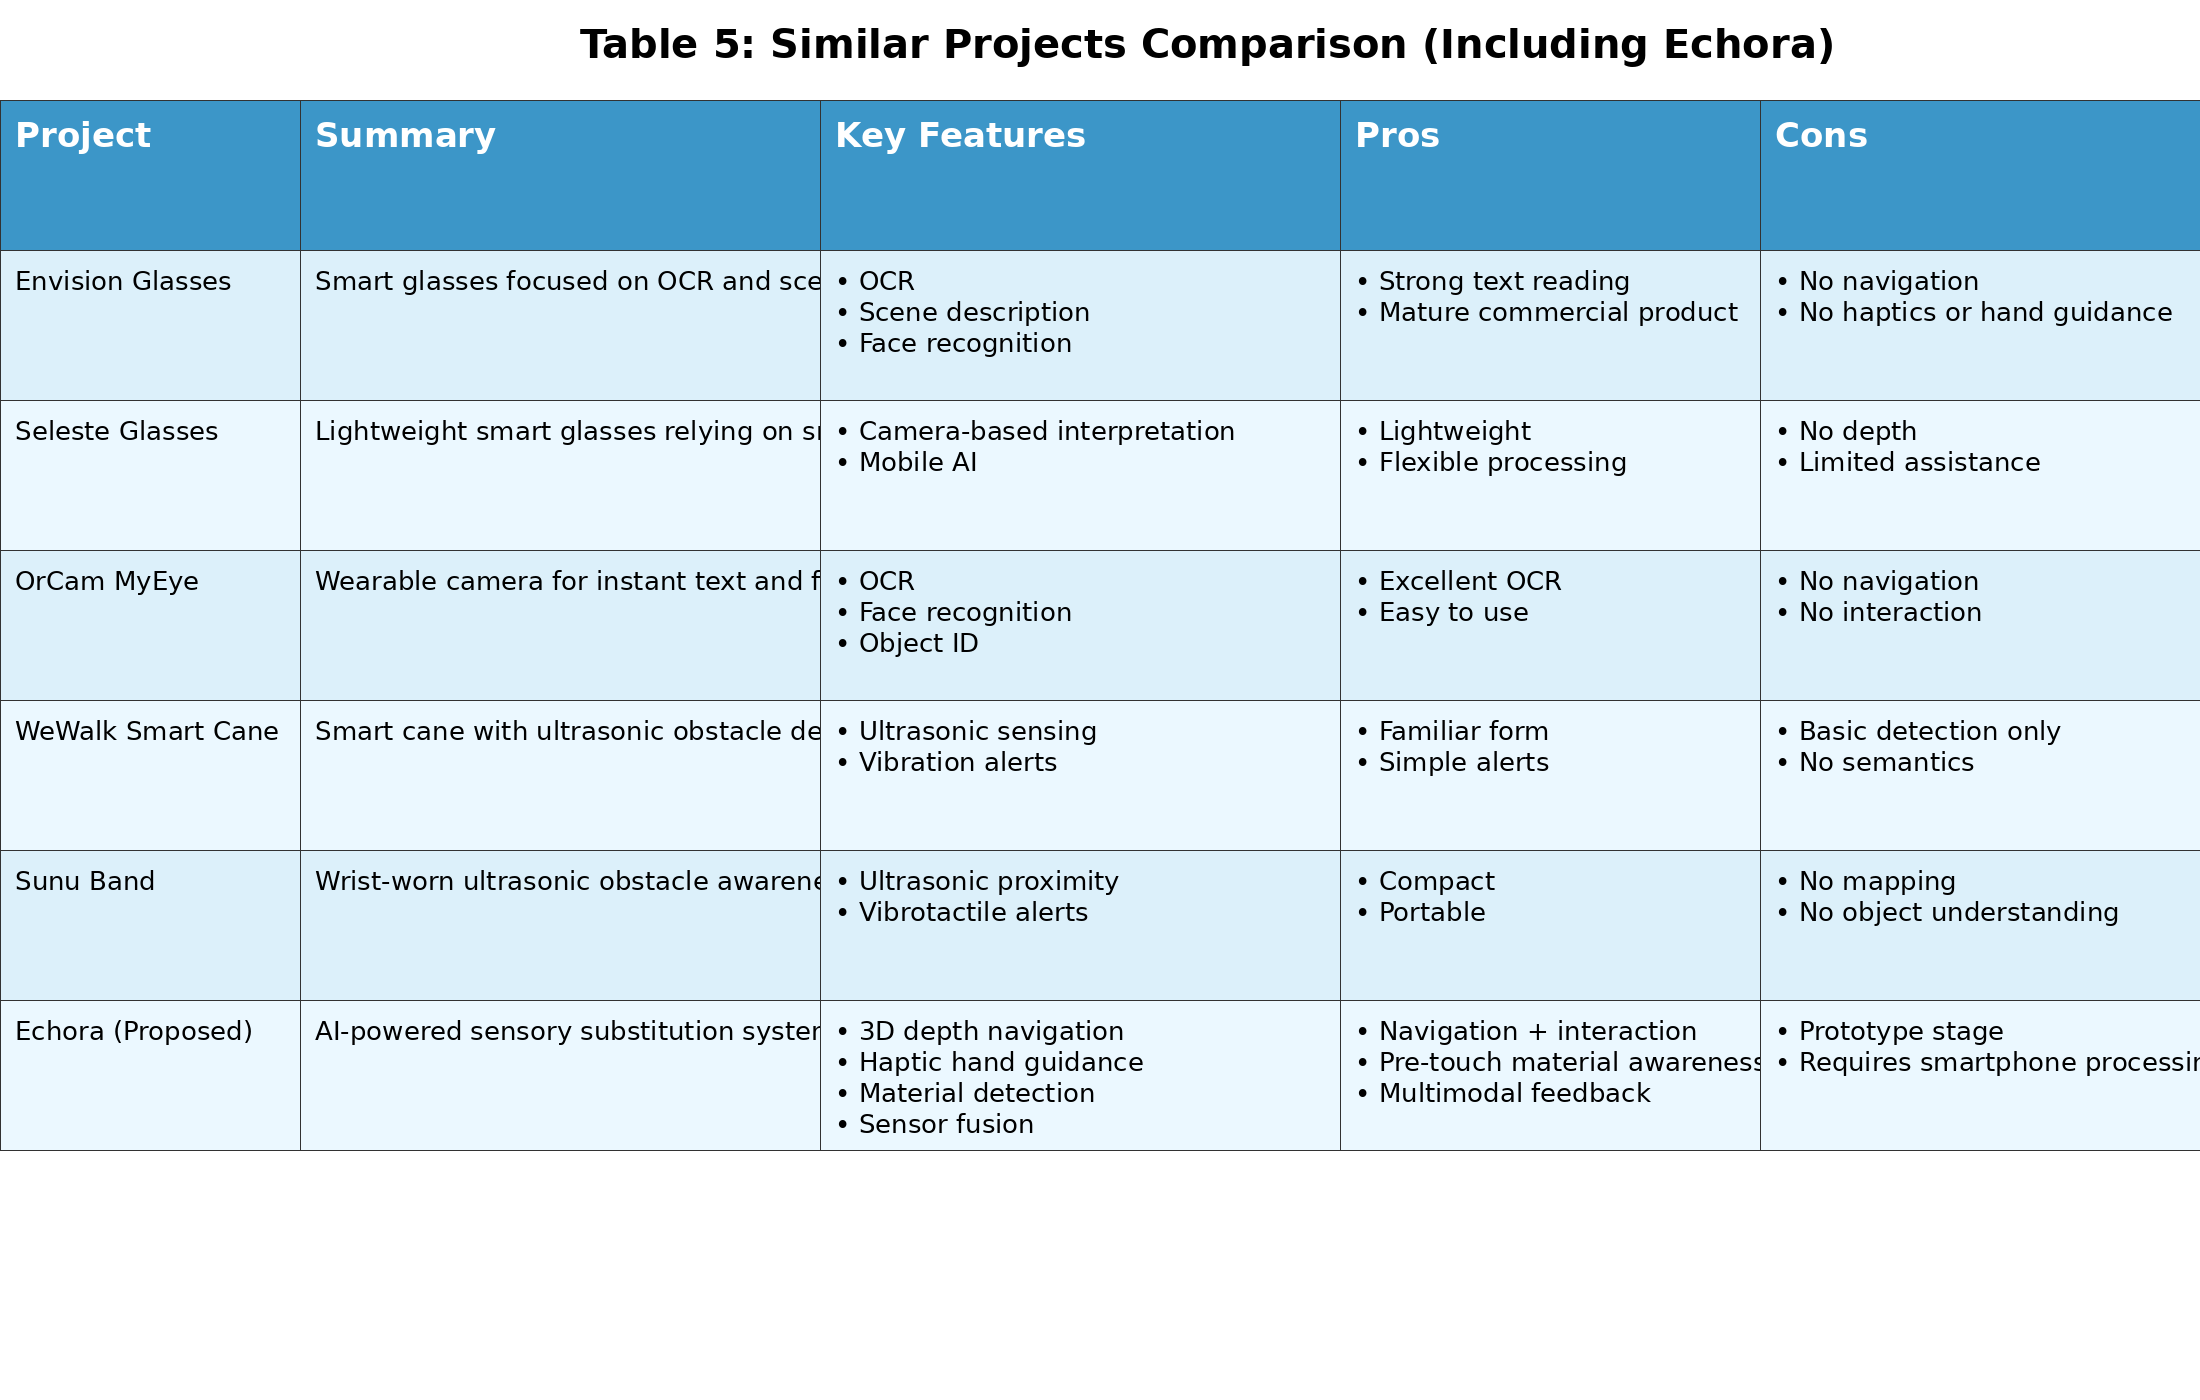
\includegraphics[width=\textwidth,keepaspectratio]{comparison.png}
\source{Teamwork}
\end{table}

\section{Research on Sensory Substitution}

The academic literature helps explain \emph{why} these gaps matter and how they might be closed. It is worth noting at the outset that sensory substitution is not just a theory: controlled studies have shown that dedicated devices can support real navigation even in people who have been blind since birth, which is what makes the approach a credible foundation for a practical aid (Chebat et al., 2011).

\textbf{Turning space into sound.} A recurring theme is converting spatial layout into continuous audio rather than occasional spoken warnings. EchoSee builds a live 3D model of the surroundings and places virtual sound sources on nearby surfaces, producing a spatial ``soundscape''; its feasibility testing reported a large reduction in collisions of around 40\%. This supports a design choice in Echora: a continuous, direction-aware sound-world can help more than a stream of discrete alerts. Easy-Access SoundView takes a simpler route, mapping vertical position to pitch and depth to loudness. Its value is the finding that \emph{minimal, well-chosen} audio codes are quick to learn, a useful reminder that more information is not always better when the user is trying to move and think at the same time (Schwartz, King and Bell, 2024; Neugebauer et al., 2020).

\textbf{Reliable models of the world.} Continuous audio is only as good as the spatial model behind it. Work on dense RGB-D mapping shows that combining depth with visual feature tracking keeps a 3D model stable even in poor lighting or on plain, low-texture surfaces. This directly justifies Echora's use of an RGB-D (colour-plus-depth) camera rather than a plain webcam: the depth channel is what makes distance zoning and safe navigation possible (St\"uckler et al., 2015).

\textbf{Feedback through touch.} A broad review of haptic wearables groups them into sensory replacement, augmentation, and training devices, and shows that vibration on the body can carry direction and urgency while easing the load on hearing. Because a BLV user relies heavily on hearing for the world around them, moving some cues onto the skin is sensible; this motivates Echora's wrist-worn vibration array for directional guidance and danger pulses (Shull and Damian, 2015).

\textbf{The hand's point of view.} Most assistive systems watch the scene from the head. \emph{Seeing With the Hands} (CHI~2025) argues that the hand is an ergonomic and flexible place to sense from, and renders tactile images onto the back of the hand so users can explore objects by touch. Importantly, participants preferred \emph{combining} an overview (eye) view with a close-up (hand) view. This finding shaped one of Echora's core design decisions: separating broad ``macro'' awareness (navigation and recognition from the head camera) from fine ``micro'' interaction (guiding the hand to a target) (Teng et al., 2025).

\textbf{OCR glasses and their limits.} Prototype OCR smart-glasses confirm that reading text on the move is valuable, but also flag practical constraints: limited language support, a narrow effective reading distance, and comfort issues when mounting a camera on the head. These lessons fed directly into Echora's text-reading design, which adds image pre-processing to cope with poor lighting and skew and only reads when text is stable and close (Envision, 2026b).

\textbf{Deep learning on wearables.} Finally, recent wearable recognition systems show that modern object detectors can run at practical speed and accuracy when models are kept lightweight and sensors are combined. This gives confidence that real-time, local inference, rather than cloud processing, is realistic, and supports Echora's decision to fuse depth and vision on a nearby computer (Lin et al., 2019; Chen, Shen and Sawada, 2023).

\section{Technical Background}

It is also worth briefly grounding the technologies that make an integrated system possible, since these underpin every design choice in the chapters that follow. Modern assistive perception rests on a small number of mature building blocks. \emph{Convolutional neural networks} (CNNs) are very good at pulling meaningful features out of images, and detectors built on them, such as the YOLO family used here, can now find and label many objects in a single fast pass, which is what makes real-time obstacle awareness realistic. \emph{Depth sensing}, whether from stereo cameras or other RGB-D sensors, adds the missing third dimension, letting a system reason about how far away things are rather than only what they are; this is essential for turning a detection into a safe/warning/danger judgement.

\emph{Sensor fusion} ties these together. By combining colour, depth, and motion (from an inertial sensor), a system can be more robust than any single input allows; for instance, using motion to decide the user is walking and should not be interrupted by a reading prompt. Finally, non-visual output relies on mature \emph{text-to-speech} and \emph{vibrotactile} techniques, where the design challenge is less about the raw technology and more about presenting information simply, in the right order, and without overwhelming the user. The recurring theme across the literature is that none of these pieces is individually novel; the difficulty, and the opportunity, lies in fusing them into a low-latency, intuitive whole that runs on affordable hardware.

\section{The Gap and How Echora Responds}

Two clear conclusions emerge from this review. First, the market is split down the middle: products either understand meaning or understand space, rarely both, and almost none add touch. Second, the research points toward an answer: fuse depth and vision for a stable model, deliver continuous spatial cues, offload some feedback to the skin, and treat broad awareness and close interaction as distinct but connected tasks.

Echora is designed as a direct response to this gap. It fuses colour and depth from a single wearable camera; it delivers information through both audio and wrist-based haptics; it unifies navigation, reading, face recognition, banknote identification, and hand-guidance under one controller; and it keeps all processing local for privacy and low latency. The next chapter describes how these ideas were turned into a working system.

\chapter{Project Development}
\label{ch:dev}

This chapter explains how Echora was built. It begins with the development method the team followed, then describes the overall architecture, the five perception modes, the safety-first controller, and the audio and haptic feedback. It closes with the physical hardware build and the datasets used to train the custom AI models. The goal is to show not only \emph{what} was built but \emph{how} the work was carried out.

\section{Development Methodology}

Echora is a real-time, safety-critical system, so the team used a user-centred, iterative approach that borrows from systems engineering, human-centred design, and Agile software development. Rather than treating navigation, reading, and interaction as unrelated problems, the project treated sensing, processing, and feedback as one tightly connected pipeline.

Work began by turning user needs into concrete requirements, drawing on the difficulties BLV users face, on safety and accessibility considerations, and on the gaps identified in the market and literature review. The system was then broken into independent modules, namely sensing, perception, decision-making, and feedback, so that each part could be developed and tested on its own before being joined to the rest. Development proceeded in short iterations: each cycle added a limited feature, tested it, and folded the lessons back into the next cycle. This exposed performance bottlenecks and usability problems early, when they were still cheap to fix.

The team managed this with Agile practices, using a prioritised backlog and sprint-based delivery across two phases: a documentation phase (requirements, specification, and design) and an implementation phase (development, integration, testing, and optimisation). Two principles ran through every iteration. The first was real-time performance as a hard requirement, not an afterthought: latency, frame rate, and resource use were monitored continuously. The second was managing the user's mental load, keeping feedback simple, non-overlapping, and always led by safety.

\section{Requirements}

Before any code was written, the team turned the user needs into concrete, testable requirements, because a safety-critical assistive device cannot be judged on features alone; it has to meet firm performance and safety targets.

The \emph{functional} requirements describe what the system must do. Navigation must acquire and fuse depth and colour data, detect and track navigation-relevant objects at a minimum of 15 frames per second, compute each object's distance and direction, and sort it into danger, warning, and safe zones, with the closest hazard always given priority. Text reading must detect text regions, run OCR with pre-processing for noise and poor lighting, and speak stable results, activating automatically when text is held close to the camera. The remaining functions, namely face recognition, banknote identification, and hand guidance, each have their own activation conditions and confirmation rules, and every mode must be reachable both automatically and by a simple manual override.

The \emph{non-functional} requirements set the quality bar. Real-time performance is treated as a hard limit: per-frame processing under about 40 milliseconds, recognition feedback under roughly 120 milliseconds, danger alerts under 100 milliseconds, and mode switches within about 200 milliseconds, so that feedback never feels laggy or unsafe. Security and privacy requirements mandate that all processing happens locally, that biometric data is handled under a privacy-by-design approach, and that sensitive features such as face recognition require explicit user consent. Reliability requirements call for graceful degradation: if depth data is lost, the system should warn the user and fall back to a simpler mode rather than fail silently. Usability requirements stress that feedback must be simple, non-overlapping, and interruptible, and that the wearable must stay comfortable for long periods. These targets guided the design decisions described in the rest of this chapter and the tests reported in Chapter~\ref{ch:results}.

\section{System Architecture}

Echora uses a distributed architecture that separates \emph{sensing and feedback} from \emph{computation and intelligence}. On the body, the user wears the sensing camera and a wrist-worn haptic module. The heavy AI work runs on a connected computer. This split keeps the wearable parts light and lets the software be upgraded without touching the hardware.

At the centre is a continuous frame loop, illustrated in Figure~\ref{fig:pipeline}. On every cycle the system: (1) captures a synchronised colour image, depth map, and motion sample from the camera; (2) runs obstacle detection on the frame and updates lighter background probes for text, faces, banknotes, and reachable objects; (3) asks the state machine\footnote{A state machine is the control logic that decides which mode Echora is in at any moment and when it is allowed to switch to another.} which mode should be active; (4) runs that mode's handler; and (5) sends the result to the user as speech, spatial sound, or vibration. Expensive operations such as text reading and face recognition run on background threads so they never stall the main loop, and results are cached where possible. The system automatically uses a GPU when one is available and falls back to the CPU otherwise. Every threshold, model path, and timing value lives in a central configuration file, so behaviour can be tuned without changing code.

Echora is written in Python and brings together a number of established open-source components. Sensing uses the DepthAI library for the Luxonis OAK-D depth camera\footnote{The OAK-D is the Luxonis stereo depth camera used as Echora's main sensor: it captures both a normal colour image and a per-pixel distance map.}. Detection and tracking use Ultralytics YOLOv8 with its built-in ByteTrack tracker\footnote{ByteTrack is a tracking method that follows the same detected object across successive frames, so it keeps one identity instead of being re-detected as a new object each frame.}, running on the PyTorch deep-learning runtime, with image handling by OpenCV. Text reading uses PaddleOCR\footnote{PaddleOCR is the open-source OCR engine used for reading text; PP-OCRv4 is the specific model version fine-tuned for this project.}; face recognition uses InsightFace; and hand tracking uses MediaPipe Hands. Speech is produced offline with pyttsx3 and alert tones with pygame, while identities and event logs are stored locally through SQLAlchemy and SQLite. An optional local vision-language model, Gemma, served through Ollama, can add short scene descriptions when the path is clear (Luxonis, 2019; Ultralytics, 2023; PyTorch, 2016; OpenCV, 2000; PaddlePaddle, 2020; DeepInsight, 2017; Google, 2019; Bhat, 2017; Pygame, 2000; SQLAlchemy, 2006; Google, 2024; Ollama, 2023).

\begin{figure}[H]
\centering
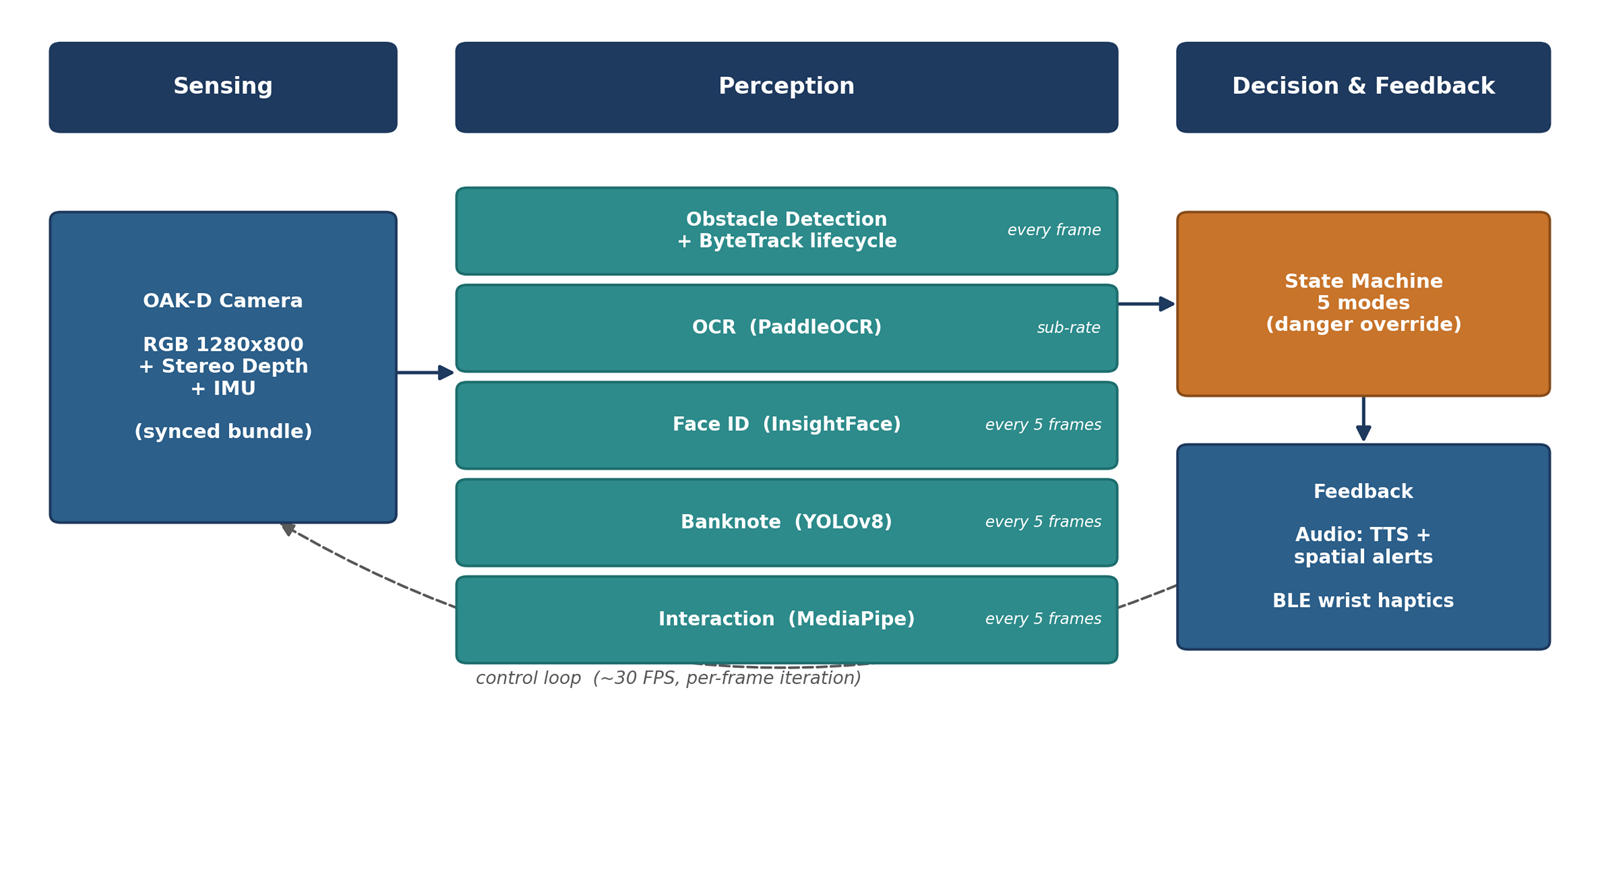
\includegraphics[width=\textwidth,keepaspectratio]{pipeline.png}
\caption{The Echora pipeline: from the camera's colour-plus-depth frame, through mode routing in the control unit, to the per-mode AI engines and the audio and haptic feedback delivered to the user.}
\label{fig:pipeline}
\source{Teamwork}
\end{figure}

\section{The Five Perception Modes}

Echora's usefulness comes from five perception modes, each handling one everyday task.

\subsection{Navigation}
Navigation is the default and most safety-critical mode. A YOLOv8 object detector runs on every frame and follows objects across frames using ByteTrack, so the same chair keeps the same identity even if it is briefly hidden. Detections are limited to navigation-relevant classes such as people, furniture, doors, and stairs. For each object, the system reads its distance from the depth map and sorts it into a zone: \emph{danger} within 1.5 metres, \emph{warning} between 1.5 and 3 metres, and \emph{safe} beyond that. Objects heading into the user's forward path are treated as more urgent. A thin ``track lifecycle'' layer on top of ByteTrack only trusts an object after it has been seen for several frames, drops it after it disappears for too long, and estimates whether it is approaching or moving away. The closest danger receives an urgent spoken alert, a sound panned to its direction, and a vibration pulse.

\subsection{Text Reading (OCR)}
The reading mode uses PaddleOCR (PP-OCRv4) with a fine-tuned English model. Before running the expensive recognition step, a quick check decides whether readable text is even present and how far away it is. Images are then cleaned adaptively, using contrast correction for dark scenes, gamma correction for bright ones, denoising, and sharpening, so that text stands out. Low-confidence or tiny detections are thrown away, and a stability buffer makes sure text is read only when it appears consistently across several frames, which prevents the system from blurting out momentary misreads. If nothing readable is found for about five seconds, the user is gently prompted to adjust the distance or angle.

\subsection{Face Recognition}
Face recognition uses InsightFace, which detects a face (RetinaFace) and turns it into a 512-number embedding (ArcFace).\footnote{RetinaFace and ArcFace are deep-learning models from the InsightFace library, for detecting faces and for converting them into embeddings respectively. An embedding is a fixed-length list of numbers, here 512 values, that represents a face so that two faces can be compared numerically.} The live embedding is compared with saved ones using cosine similarity, and a match is only accepted if it is both strong enough and clearly ahead of the second-best candidate, a rule that cuts down false identifications. A light-weight probe runs during navigation to save computation, and full recognition only fires when a face is actually present and stays stable across frames. Enrolling a person is a deliberate step: the user types a name, the system captures a short burst of good-quality frames, averages the best embeddings, and stores the result. Providing that name is treated as the user's consent to store the identity.

\subsection{Banknote Identification}
Handling cash is a common worry for BLV users, so Echora includes a dedicated Egyptian Pound detector, a custom YOLOv8 model covering eleven classes of notes and coins, including the newer note designs. To be sure the user is actually holding a note, detections are only accepted at close range and above a high confidence threshold, and a short history buffer confirms the denomination before it is announced once. A cooldown then stops the same note being read again immediately.

\subsection{Hand Guidance (Interaction)}
The interaction mode helps the user physically reach an object such as a handle or a lift button. It combines MediaPipe Hands, which tracks 21 points on the hand, with the existing YOLO detections. The system measures the gap between the fingertip and the target in three directions, namely left/right, up/down, and depth, and moves through guidance phases (idle, guiding, edge, success) as the hand closes in. The direction is turned into a vibration pattern on the wristband, growing stronger as the hand approaches, with a distinct confirmation buzz when the target is reached.

\section{Safety-First State Machine}

With five modes available, the system needs a reliable way to choose between them. This is the job of the context-aware state machine, summarised in Figure~\ref{fig:state_machine}. It watches the perception results and the motion sensor and switches mode accordingly: stable text within reach while the user is still triggers reading; a nearby reachable object triggers hand guidance; a confidently recognised face triggers face mode; and so on. To stop the system flickering between modes, each switch must persist for several frames, and each mode must stay active for a minimum time before it can be left.

Above all of this sits one non-negotiable rule: if a danger-zone obstacle appears, the system immediately returns to navigation, whatever it was doing. Safety always wins. This single override is what makes it acceptable for the system to spend time reading a sign or identifying a note: the moment something becomes dangerous, that activity is dropped.

\begin{figure}[H]
\centering
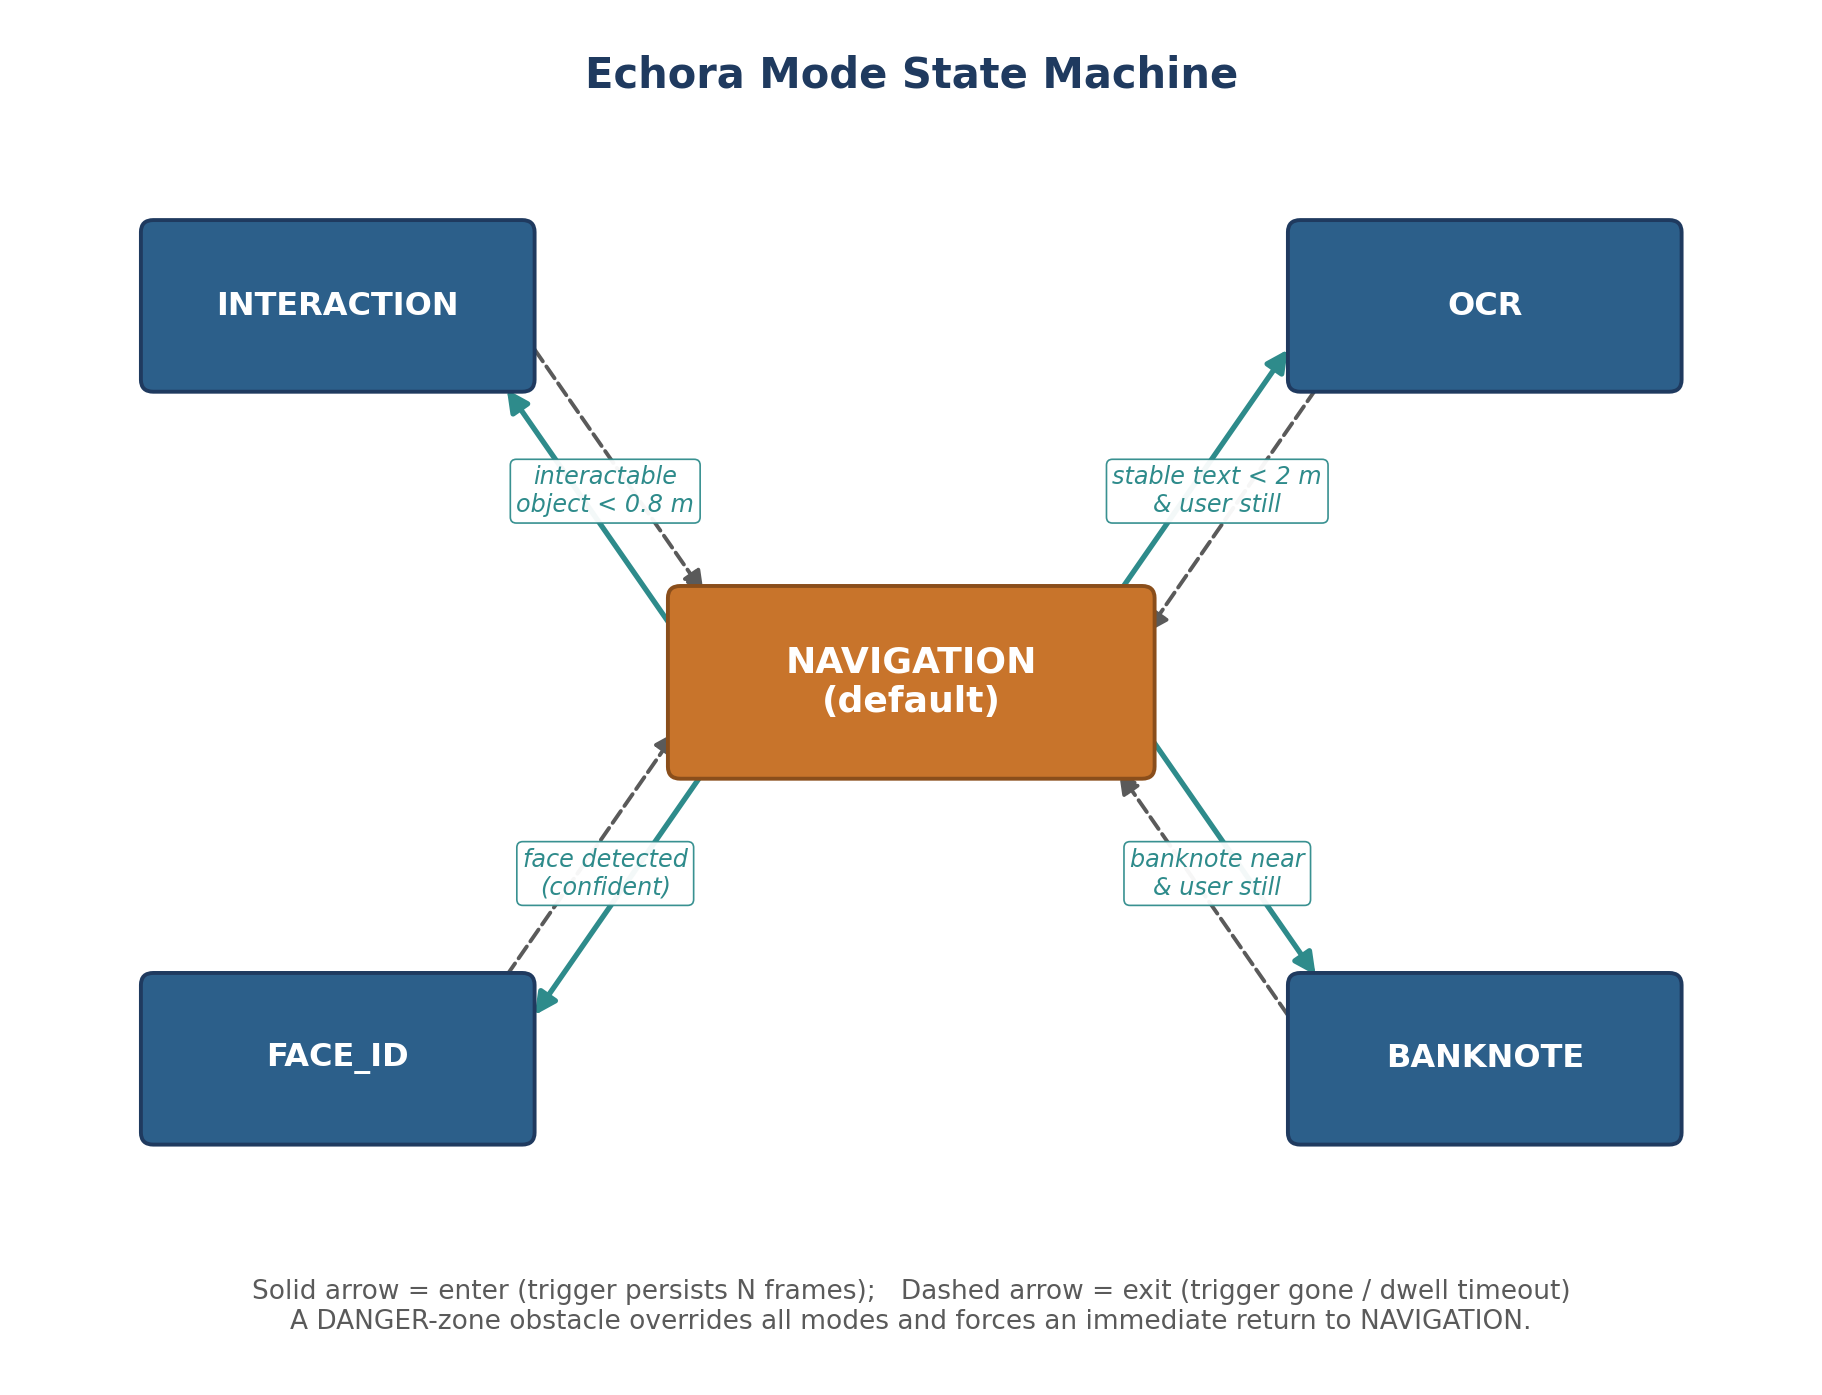
\includegraphics[width=\textwidth,keepaspectratio]{state_machine.png}
\caption{Echora's mode state machine: triggers (solid) and exits (dashed) around the default navigation mode, with the danger override returning control to navigation from any mode.}
\label{fig:state_machine}
\source{Teamwork}
\end{figure}

\section{Audio and Haptic Feedback}

Because the user cannot see the screen, feedback design is central rather than cosmetic. Audio uses offline text-to-speech so that no internet is needed. Messages go into a priority queue, so an urgent obstacle warning can jump ahead of a routine announcement, and a watchdog restarts the speech worker if it ever stalls. Alert tones are panned left or right to match an object's direction, giving an intuitive sense of where it is, and short cooldowns stop the same cue repeating too often.

Haptic feedback is delivered through the wrist module. Directional and proximity patterns, together with a dedicated success pattern for hand guidance, are generated on background threads so that touch output never blocks the perception loop. The hardware behind this is described next.

\section{Hardware Build}

Echora was not only software; it was built as a wearable prototype. Two devices were made in parallel: the head unit carrying the camera, and the wrist-worn haptic module.

The head unit began as a 3D model in SolidWorks, designed against a reference head so that fit, weight balance, and the camera's field of view could be checked before anything was printed. The enclosure was then 3D-printed in parts, which house the depth camera behind a front bezel along with lithium cells, wiring, and a power switch. Because printed parts show visible layer lines, each surface was filled, wet-sanded, primed, and spray-painted for a smooth, finished look, and the Echora brand mark was applied. The result, shown in Figure~\ref{fig:hardware}(a), is a comfortable, adjustable headset that looks like a real product rather than a bench prototype.

The haptic module was developed as a separate hardware track. The driver circuit was first prototyped on a breadboard and then committed to a custom printed circuit board. A clever detail keeps the design simple: twenty coin vibration motors are driven from just three microcontroller pins by cascading three 74LS595 shift registers into three ULN2803A driver arrays. The 5\,V control logic and the 3.7\,V motor supply are kept on separate power rails that share only a common ground, so the current spikes from the motors cannot brown out the ESP32 controller.\footnote{The ESP32 is a low-cost Wi-Fi microcontroller; here it drives the wristband's vibration motors.} The finished, self-contained module is shown in Figure~\ref{fig:hardware}(b).

\begin{figure}[H]
\centering
\begin{minipage}[b]{0.48\textwidth}\centering
  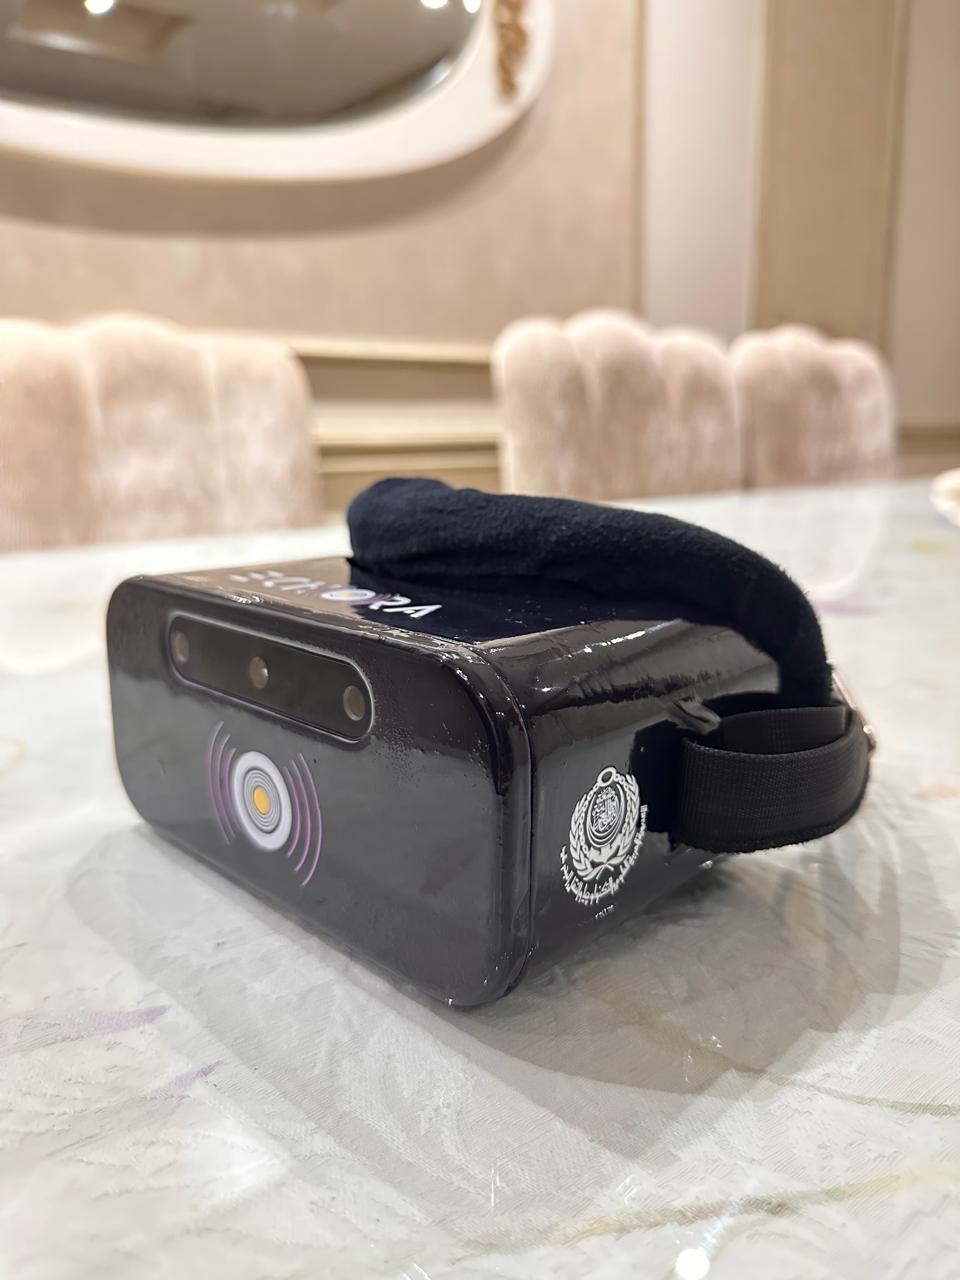
\includegraphics[width=\linewidth,height=5.2cm,keepaspectratio]{hardware_glasses.jpeg}\\[2pt]
  {\footnotesize (a) The finished head unit}
\end{minipage}\hfill
\begin{minipage}[b]{0.48\textwidth}\centering
  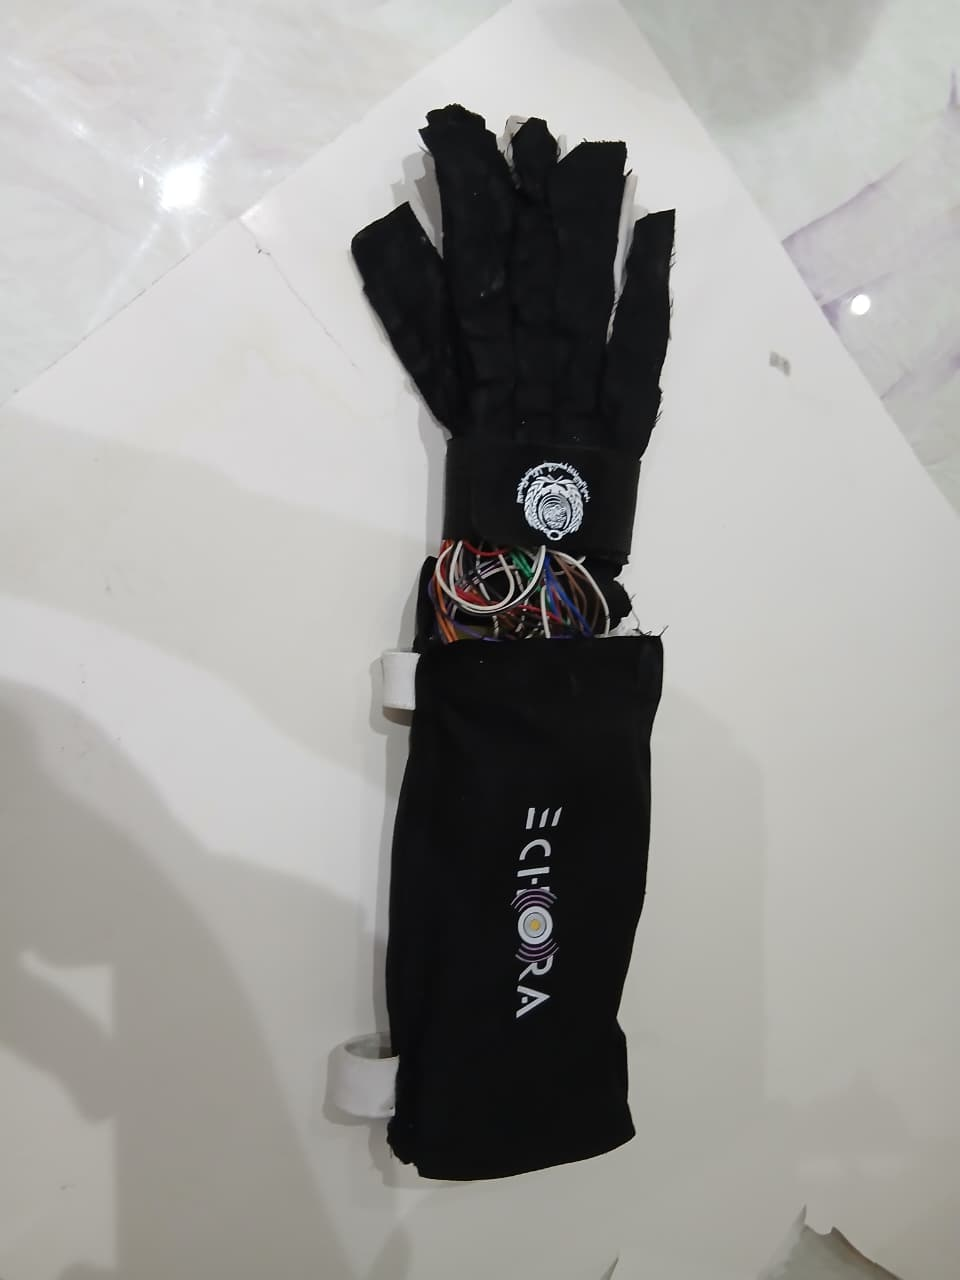
\includegraphics[width=\linewidth,height=5.2cm,keepaspectratio]{hardware_wristband.png}\\[2pt]
  {\footnotesize (b) The wrist-worn haptic module}
\end{minipage}
\caption{The two wearable devices built for the Echora prototype.}
\label{fig:hardware}
\source{Teamwork}
\end{figure}

\section{Datasets and Model Training}

Three of Echora's models were custom-trained, because off-the-shelf models did not fit the task well enough.

\textbf{Accessibility detector.} To detect doors, handles, and lift controls, two public Roboflow datasets, a door-and-handles set and a lift-button set, were merged and cleaned into a focused seven-class set (door, door handle, up, updown, close, down, open). All door images were kept, while lift images were filtered down to the five relevant control types. The combined dataset holds 2,719 images (2,156 for training, 289 for validation, and 274 for testing), shown in Figure~\ref{fig:datasets}. A YOLOv8s detector was fine-tuned from pretrained weights for 80 epochs at 640$\times$640 resolution on a GPU (UAEU, 2022; Sun Moon University, 2022).

\textbf{Egyptian banknote detector.} No suitable public dataset of Egyptian currency existed, so the team created one. It covers eleven denomination classes across notes, coins, and the newer designs, with images captured under varied lighting, backgrounds, and angles for robustness, all labelled by hand. The dataset holds more than 7,400 annotated images, split 80/10/10 (Figure~\ref{fig:datasets}), and was used to train a YOLOv8 detector (Abdelrahman, no date).

\textbf{Text recognition.} To read real-world text better than the default model, the English PP-OCRv4 recogniser was fine-tuned on a sample of the large-scale TextOCR dataset, which holds about 28,000 images and over 900,000 words. Word regions were cropped, filtered to sensible English words, and used to fine-tune the recogniser for 15 epochs (RobikScube, 2021).

\begin{figure}[H]
\centering
\begin{minipage}[b]{0.48\textwidth}\centering
  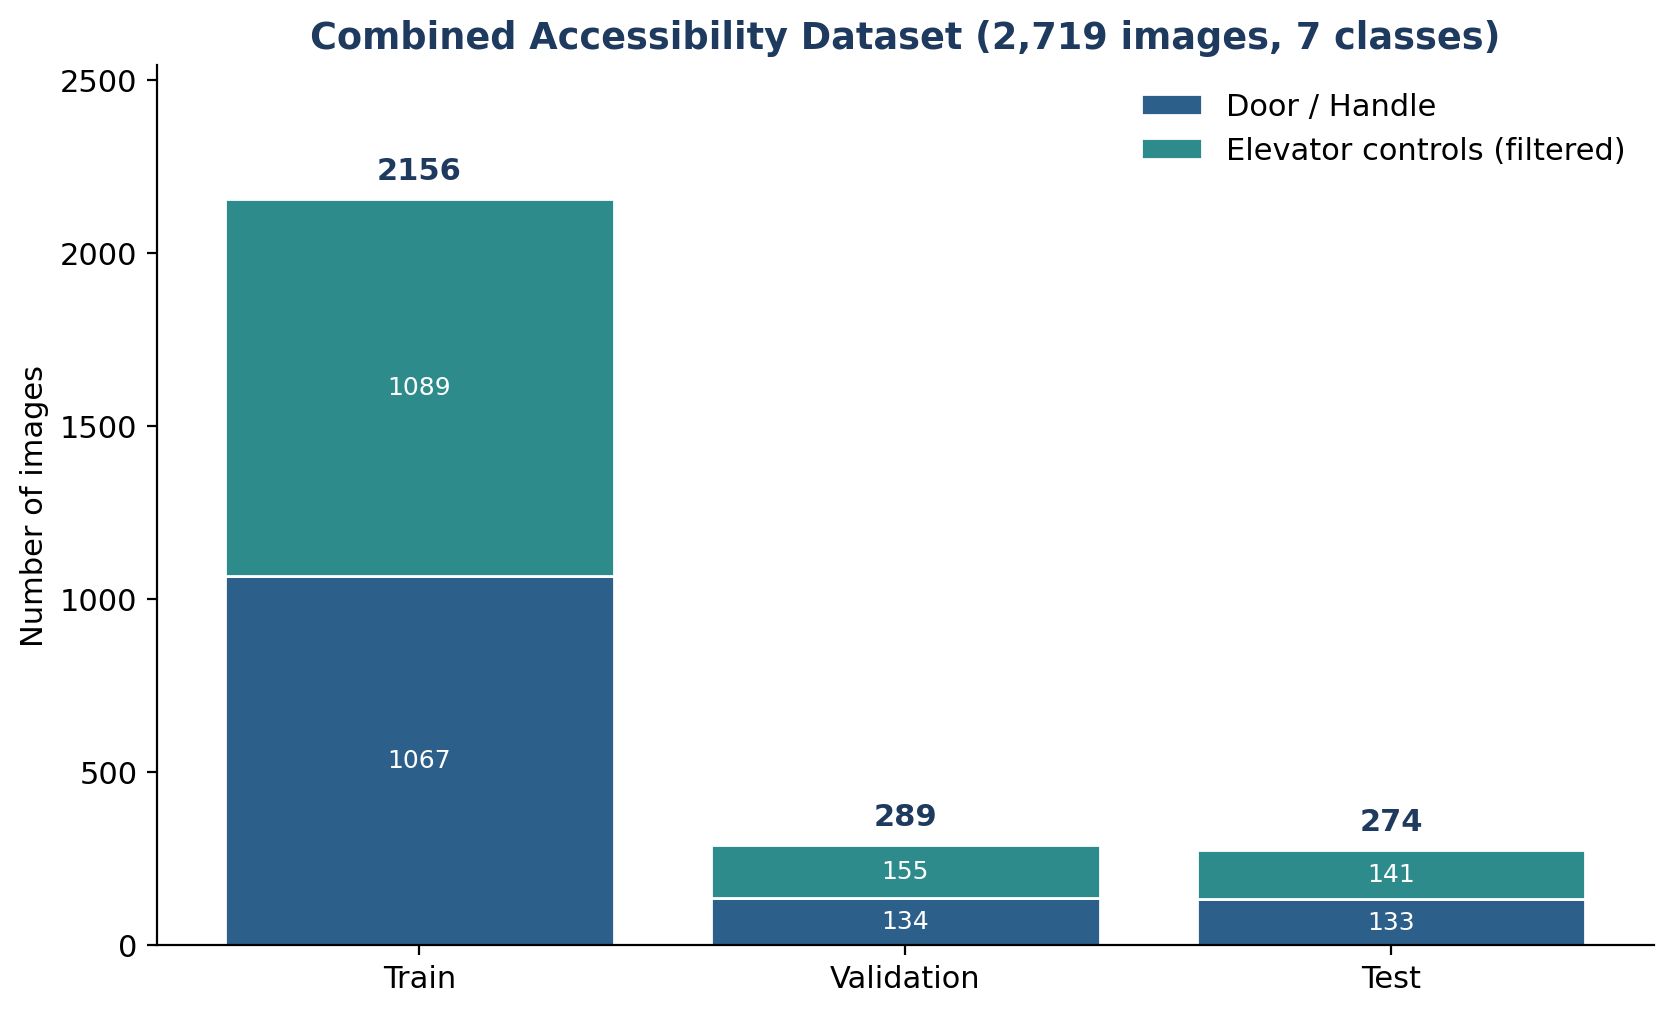
\includegraphics[width=\linewidth,keepaspectratio]{accessibility_dataset.png}\\[2pt]
  {\footnotesize (a) Accessibility dataset splits}
\end{minipage}\hfill
\begin{minipage}[b]{0.48\textwidth}\centering
  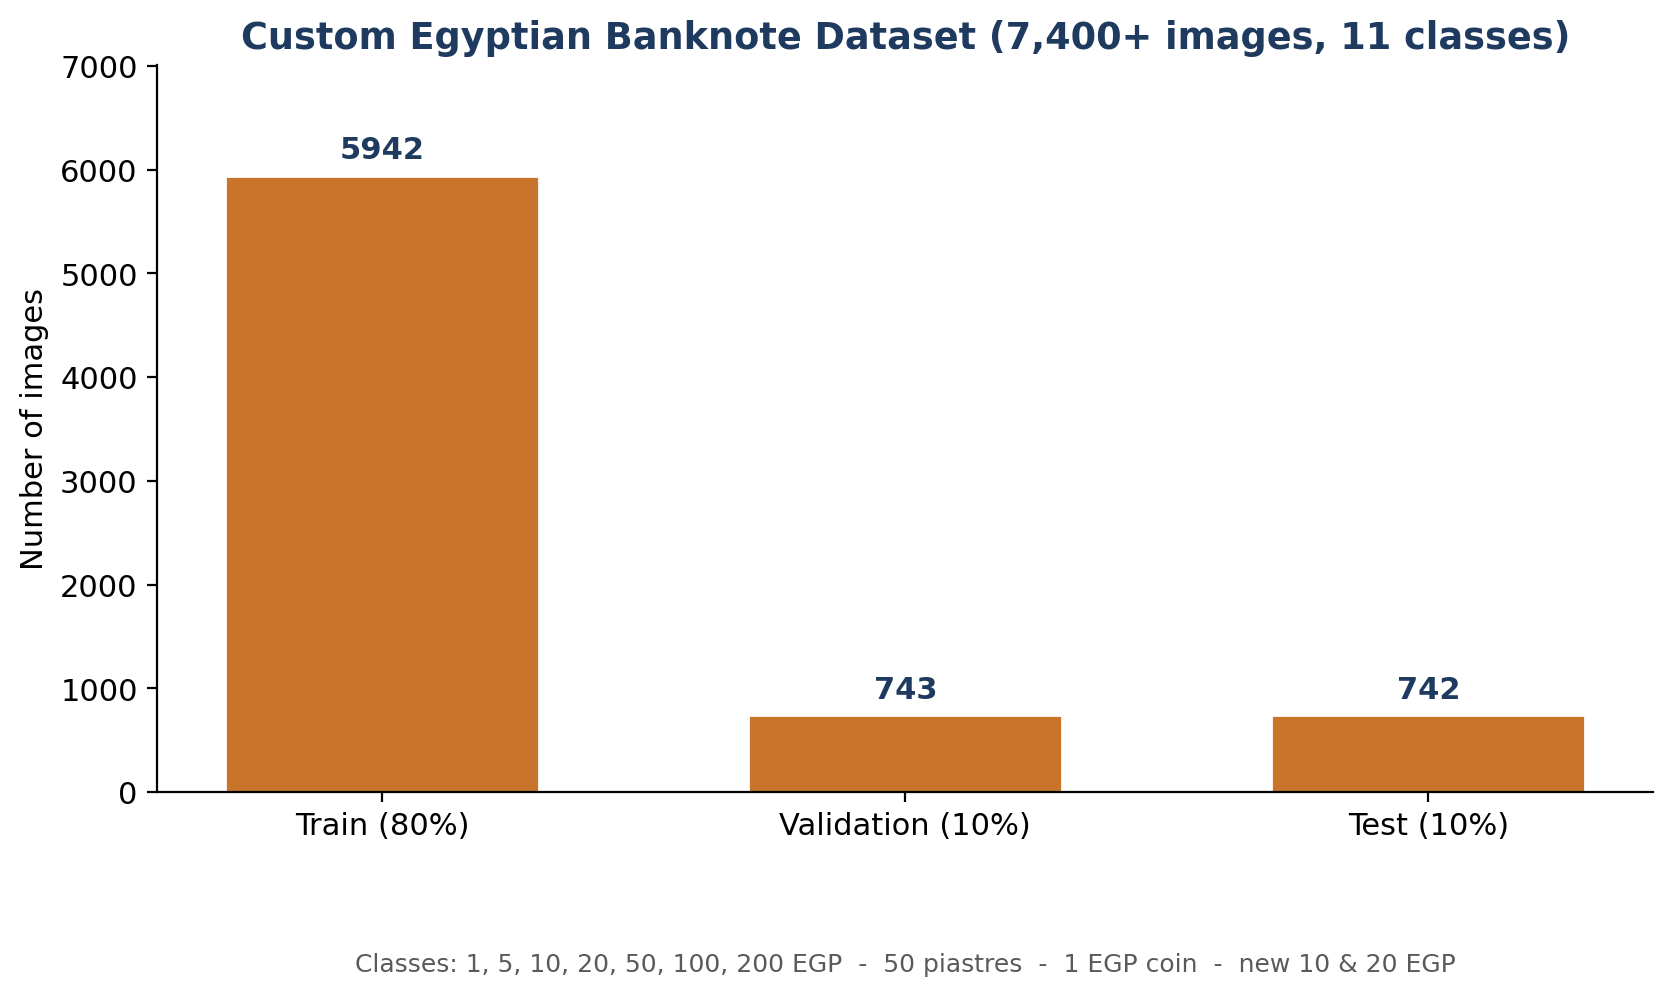
\includegraphics[width=\linewidth,keepaspectratio]{banknote_dataset.png}\\[2pt]
  {\footnotesize (b) Banknote dataset splits}
\end{minipage}
\caption{Composition of the two custom detection datasets across train, validation, and test splits.}
\label{fig:datasets}
\source{Teamwork}
\end{figure}

\section{Ethics, Privacy, and Sustainability}

Because Echora carries a camera into homes and public spaces and can recognise individual people, ethical and privacy questions were treated as design requirements, not afterthoughts. The strongest safeguard is architectural: all perception runs locally on the user's computer, and no image or face embedding is sent to any external service. Face recognition is opt-in by design: a person is only stored when the user deliberately enrols them and types a name, and that act is treated as consent. The team is honest that the current prototype stores these embeddings without encryption at rest, and adding this is listed as future work.

There is also an ethical duty to avoid over-reliance. Echora is deliberately positioned as a \emph{complement} to the white cane and guide dog, not a replacement, and it degrades gracefully so that a sensor failure produces a clear warning rather than dangerous silence. On sustainability, running inference on an ordinary computer rather than requiring specialised or cloud infrastructure keeps both cost and energy use down, and the modular, upgradeable software means the hardware need not be replaced to gain new features. These considerations align the project with the Sustainable Development Goals identified in Chapter~\ref{ch:intro}.

With the system built and the models trained, the next chapter reports how well they performed.

\chapter{Results}
\label{ch:results}

This chapter reports and critically reviews the results of the project. It looks first at the accuracy of the two custom detection models, then at how the software behaved under automated testing, and finally at how the complete system performed when run end-to-end in real time. Results are reported honestly, including the weaknesses, because a fair account of what did \emph{not} work is as useful as the headline numbers.

\section{Evaluation Method}

All detection results were produced by a single, reproducible evaluation script that runs each trained model against its held-out test split, that is, data the model never saw during training. The standard object-detection measures are used: precision (of the things the model flagged, how many were correct), recall (of the things it should have found, how many it did), and mean Average Precision at an overlap threshold of 0.5 (mAP@0.5), together with the stricter mAP averaged over overlap thresholds from 0.5 to 0.95 (mAP@0.5:0.95). Software behaviour was checked with an automated test suite, and the whole system was exercised through scripted scenarios and live camera runs.

\section{Accessibility Detection Model}

The accessibility detector was tested on its 274-image held-out split. The overall and per-class results are given in Table~\ref{tab:acc_results}, and the confusion matrix in Figure~\ref{fig:cm_acc}.

\begin{table}[H]
\centering
\caption{Accessibility detection model results on the test split (YOLOv8s).}
\label{tab:acc_results}
\begin{tabular}{lcccc}
\toprule
\textbf{Class} & \textbf{Precision} & \textbf{Recall} & \textbf{mAP@0.5} & \textbf{mAP@0.5:0.95} \\
\midrule
door & 0.866 & 0.874 & 0.913 & 0.741 \\
door handle & 0.787 & 0.758 & 0.793 & 0.444 \\
up & 0.812 & 0.755 & 0.774 & 0.623 \\
updown & 1.000 & 0.000 & 0.000 & 0.000 \\
close & 0.888 & 0.827 & 0.895 & 0.664 \\
down & 0.833 & 0.777 & 0.812 & 0.598 \\
open & 0.821 & 0.851 & 0.895 & 0.654 \\
\midrule
\textbf{All classes} & \textbf{0.858} & \textbf{0.692} & \textbf{0.726} & \textbf{0.532} \\
\bottomrule
\end{tabular}
\source{Teamwork}
\end{table}

\begin{figure}[H]
\centering
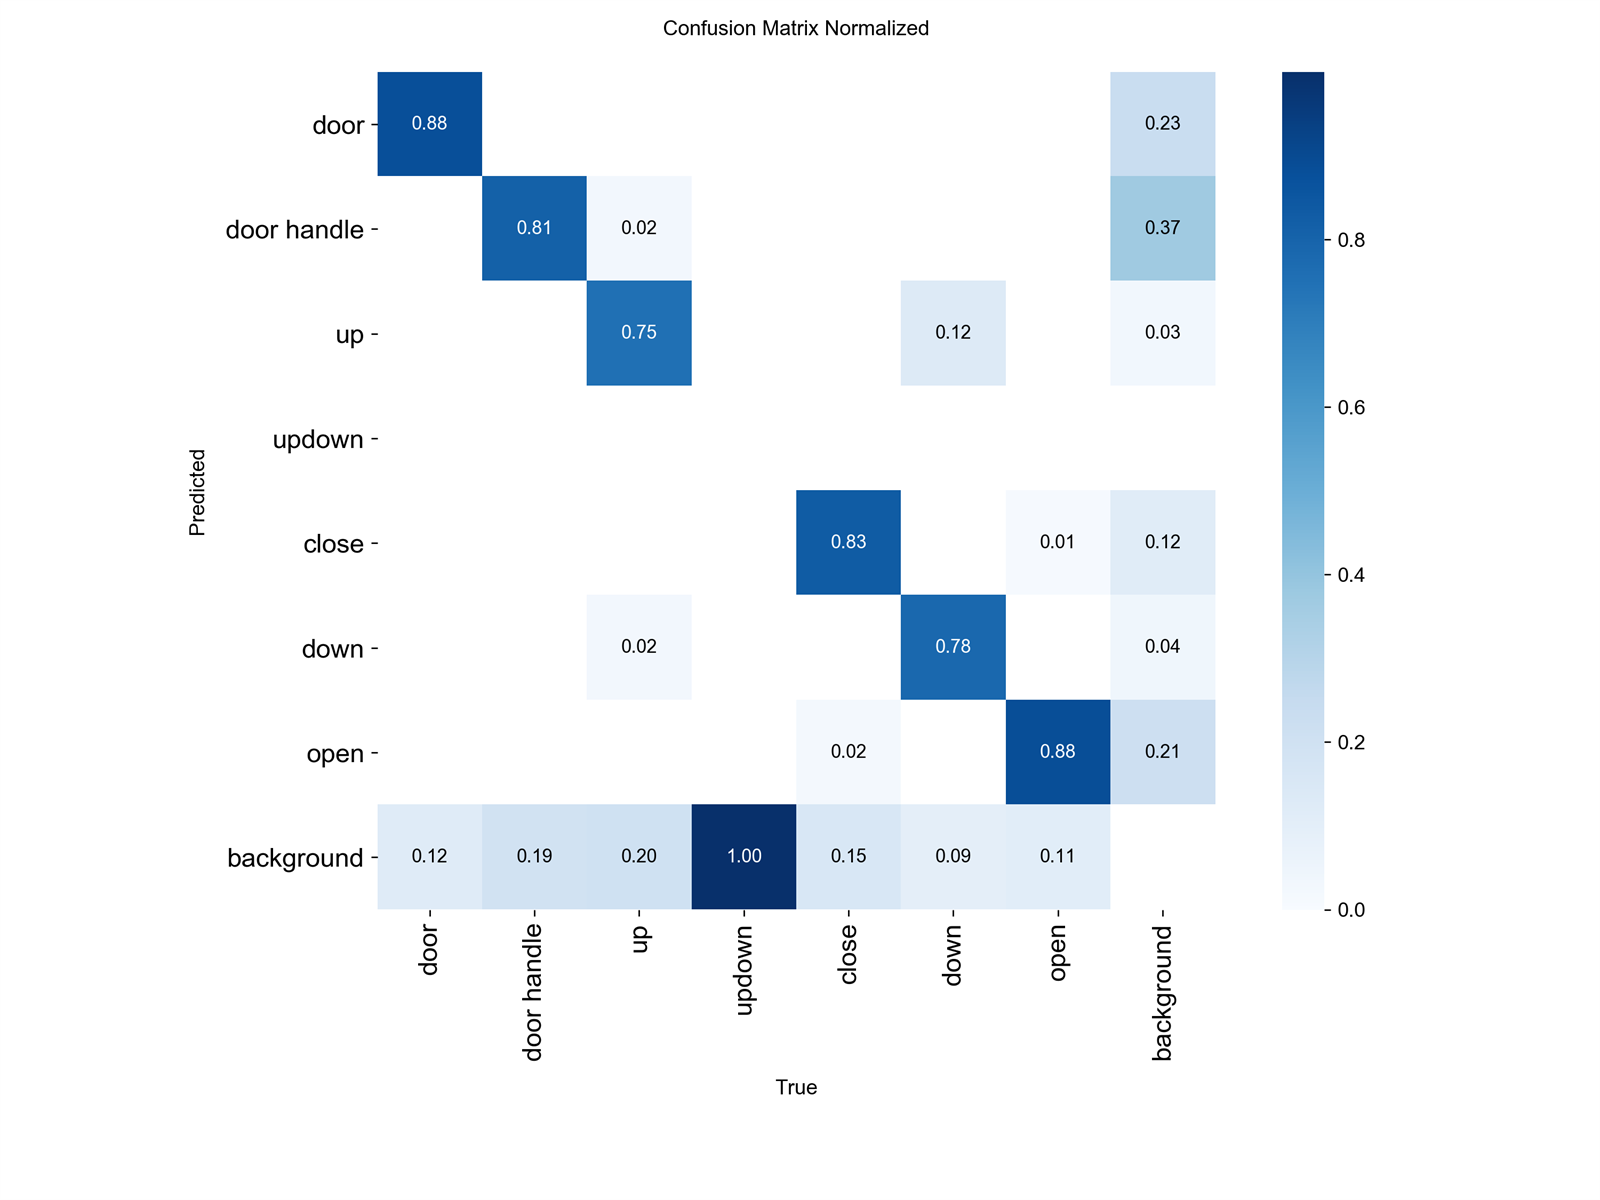
\includegraphics[width=0.72\textwidth,keepaspectratio]{cm_accessibility.png}
\caption{Normalised confusion matrix for the accessibility detection model on the test split.}
\label{fig:cm_acc}
\source{Teamwork}
\end{figure}

The model does well on the classes that matter most for safety and interaction. Doors are detected strongly (mAP@0.5 = 0.913), and the lift ``close'' and ``open'' controls both reach 0.895. Door handles are harder (0.793), which is expected: a handle is a small object and small objects are always more difficult to localise precisely. Overall the detector reaches a mean precision of 0.858 and mAP@0.5 of 0.726.

One result deserves an honest critical note. The ``updown'' class collapses to zero recall: the model finds none of its test instances. This is not a mysterious failure but a data problem: that class is severely under-represented in the split, so the model never learned it well and there are too few examples to score against. This drags the overall recall (0.692) and mAP down and is the single clearest weakness in this model. The fix is straightforward in principle: collect and balance many more ``updown'' examples and retrain. It is worth stressing that in the running system these detections are not acted on blindly; the ByteTrack lifecycle layer requires an object to be seen consistently before it is trusted, which cushions the effect of occasional per-frame errors. For the assisted-interaction use case, this level of accuracy is usable, but the class imbalance is a genuine limitation to be addressed.

\section{Banknote Detection Model}

The Egyptian banknote detector was tested on a labelled held-out set of 266 images. Its results, in Table~\ref{tab:bank_results}, are excellent.

\begin{table}[H]
\centering
\caption{Banknote detection model results on the 266-image labelled test set (YOLOv8).}
\label{tab:bank_results}
\begin{tabular}{lcccc}
\toprule
\textbf{Class} & \textbf{Precision} & \textbf{Recall} & \textbf{mAP@0.5} & \textbf{mAP@0.5:0.95} \\
\midrule
1 EGP & 0.994 & 1.000 & 0.995 & 0.981 \\
1 EGP (coin) & 1.000 & 1.000 & 0.995 & 0.986 \\
5 EGP & 0.997 & 1.000 & 0.995 & 0.982 \\
10 EGP & 0.994 & 1.000 & 0.995 & 0.989 \\
new 10 EGP & 1.000 & 1.000 & 0.995 & 0.982 \\
20 EGP & 1.000 & 1.000 & 0.995 & 0.975 \\
new 20 EGP & 1.000 & 1.000 & 0.995 & 0.974 \\
50 piastres & 0.996 & 1.000 & 0.995 & 0.990 \\
50 EGP & 0.996 & 1.000 & 0.995 & 0.984 \\
100 EGP & 0.995 & 1.000 & 0.995 & 0.995 \\
200 EGP & 0.997 & 0.960 & 0.955 & 0.936 \\
\midrule
\textbf{All classes} & \textbf{0.997} & \textbf{0.996} & \textbf{0.991} & \textbf{0.979} \\
\bottomrule
\end{tabular}
\source{Teamwork}
\end{table}

The detector achieves near-perfect performance: an overall mAP@0.5 of 0.991, precision of 0.997, and recall of 0.996. Every denomination scores at least 0.955, and the confusion matrix (Figure~\ref{fig:cm_bank}) is almost purely diagonal, meaning notes are very rarely confused with one another, which is exactly what a user needs when the difference between two notes is real money. The only visible weakness is a small fraction of 200~EGP notes that go undetected (counted as background), reflected in that class's slightly lower recall of 0.960.

\begin{figure}[H]
\centering
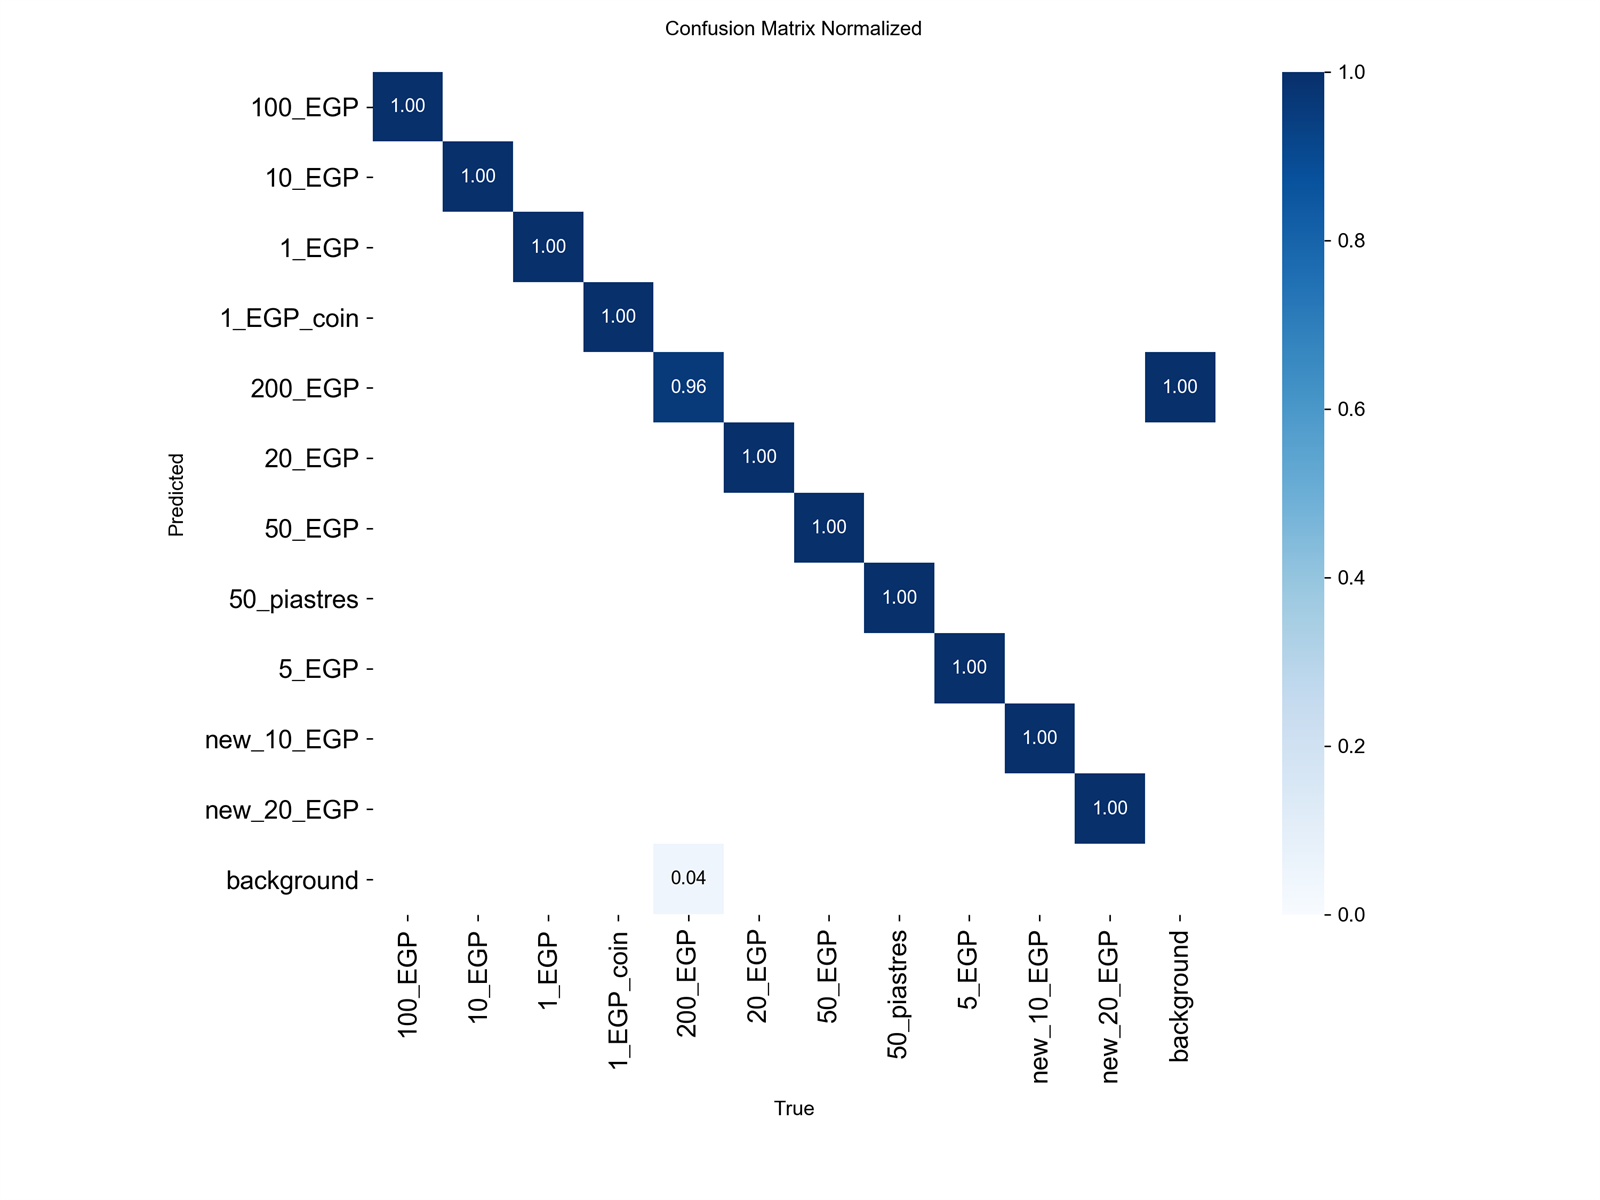
\includegraphics[width=0.72\textwidth,keepaspectratio]{cm_banknote.png}
\caption{Normalised confusion matrix for the banknote detection model on the labelled test set.}
\label{fig:cm_bank}
\source{Teamwork}
\end{figure}

These strong numbers should be read with a little caution. The banknotes were photographed by the team, so the test set, while unseen during training, comes from a similar setting; performance on very different lighting, worn notes, or unusual angles may be lower. Even so, the near-perfect scores and the clean confusion matrix give real confidence that the custom dataset and detector are well matched to the task, and they clearly show the value of building a dataset specifically for the problem rather than relying on a generic model.

\section{Qualitative Results for the Other Modes}

The two detection models above can be scored with precise numbers because they have labelled test sets. The remaining modes, namely text reading, face recognition, and hand guidance, are harder to reduce to a single figure, so they were assessed qualitatively through their automated tests and live runs. Their results are reported here honestly, as observations rather than headline metrics.

\textbf{Text reading.} With the fine-tuned English model and the adaptive pre-processing pipeline, the reader handled clear, well-lit printed text reliably and spoke it in a sensible reading order. The stability buffer proved its worth in practice: by only reading text seen consistently across several frames, it stopped the system blurting out momentary misreads as the camera moved. The honest limitations are those flagged in the OCR-glasses literature: performance drops on small, distant, low-contrast, or steeply angled text, which is why the mode only activates when text is close and the user is still, and prompts the user to reposition if nothing readable is found.

\textbf{Face recognition.} The two-part matching rule, which requires both a strong similarity score and a clear margin over the second-best candidate, worked as intended in testing, reducing the chance of confidently naming the wrong person, which is the most damaging error this mode can make. Requiring a stable identity across several frames before speaking further reduced false announcements. The trade-off is that recognition is deliberately cautious: a briefly glimpsed or poorly lit face is more likely to be reported as ``unknown'' than guessed at, which for an assistive device is the safer failure.

\textbf{Hand guidance.} The interaction mode successfully translated the three-dimensional gap between the fingertip and a target object into directional vibration, moving through its guidance phases and firing a distinct confirmation pattern on success. Because it reuses the same object detections as navigation, its ceiling is partly set by the accessibility detector's accuracy on small objects such as handles, the weakest area of that model, so guidance is smoothest for larger, clearly detected targets.

\textbf{Audio and haptic feedback.} The priority queue behaved correctly under test: urgent obstacle warnings preempted routine announcements, and per-cue cooldowns prevented the same message repeating too quickly. Directional panning gave an intuitive left/right sense of where an object was. These are usability behaviours rather than accuracy metrics, but they are central to whether the system feels calm and trustworthy rather than chaotic.

\section{Software Testing}

Alongside the models, the application software was checked with an automated integration test suite run through \texttt{pytest}. These tests exercise the perception engines on sample inputs to confirm their end-to-end behaviour. As Table~\ref{tab:sw_tests} shows, all 22 automated tests passed, covering obstacle detection, OCR, interaction, banknote logic, and audio.

\begin{table}[H]
\centering
\caption{Automated integration (pytest) test results.}
\label{tab:sw_tests}
\begin{tabular}{lcc}
\toprule
\textbf{Test group} & \textbf{Cases} & \textbf{Result} \\
\midrule
Obstacle detection (runtime) & 7 & Pass \\
OCR (runtime) & 8 & Pass \\
Interaction detection (runtime) & 4 & Pass \\
Banknote detection (runtime) & 2 & Pass \\
Audio feedback (runtime) & 1 & Pass \\
\midrule
\textbf{Total} & \textbf{22} & \textbf{All pass} \\
\bottomrule
\end{tabular}
\source{Teamwork}
\end{table}

It is worth being clear about what these tests do and do not prove. They confirm that each engine behaves correctly on controlled inputs; they do not, on their own, prove that the whole system works together on a real camera. That is the purpose of the system-level testing described next.

\section{System Integration and Real-Time Performance}

To test Echora as a whole rather than as separate parts, two complementary methods were used. First, the state machine, the component that fuses every engine's output into one behaviour, was driven through scripted multi-frame scenarios that target the cross-engine interactions no single-engine test can reach: switch debouncing, minimum dwell time, the motion gate, and the danger override. Second, the complete system was run live on the camera in furnished indoor spaces while a user moved through the scene and triggered each mode.

The scripted scenarios all passed, as summarised in Table~\ref{tab:system_tests}. Most importantly, a danger-zone obstacle always forced an immediate return to navigation, whatever mode was active, confirming that the safety path really does take precedence.

\begin{table}[H]
\centering
\caption{System-level scenarios exercising the end-to-end state-machine behaviour.}
\label{tab:system_tests}
\begin{tabular}{cp{0.42\textwidth}p{0.24\textwidth}c}
\toprule
\textbf{\#} & \textbf{Scenario} & \textbf{Expected outcome} & \textbf{Result} \\
\midrule
1 & Idle scene, no triggers & Stay in navigation & Pass \\
2 & Text visible for a single frame & No switch (debounce) & Pass \\
3 & Stable text, user still, dwell elapsed & Switch to OCR & Pass \\
4 & Danger obstacle appears while in OCR & Override to navigation & Pass \\
5 & Text visible while user walks fast & Stay in navigation (motion gate) & Pass \\
6 & Stable, confident face detected & Switch to face mode & Pass \\
7 & Every mode change recorded & Transition logged & Pass \\
\bottomrule
\end{tabular}
\source{Teamwork}
\end{table}

During the live runs, the integrated system sustained real-time operation at roughly 20--21 frames per second while detecting and tracking several obstacles at once, estimating each object's distance and bearing, and sorting it into a safe, warning, or danger zone. Figure~\ref{fig:debug} shows two representative frames from the debug view. In the first, several chairs and a couch are tracked in the warning zone, each labelled with its distance and direction. In the second, a chair that has entered the danger corridor is flagged in red while a more distant couch stays green in the safe zone. The on-screen mode, frame counter, frame rate, and per-zone counts confirm that the whole pipeline, from capture through detection and tracking, depth zoning, and state evaluation to feedback, runs together in real time.

\begin{figure}[H]
\centering
\begin{minipage}[t]{0.49\textwidth}\centering
  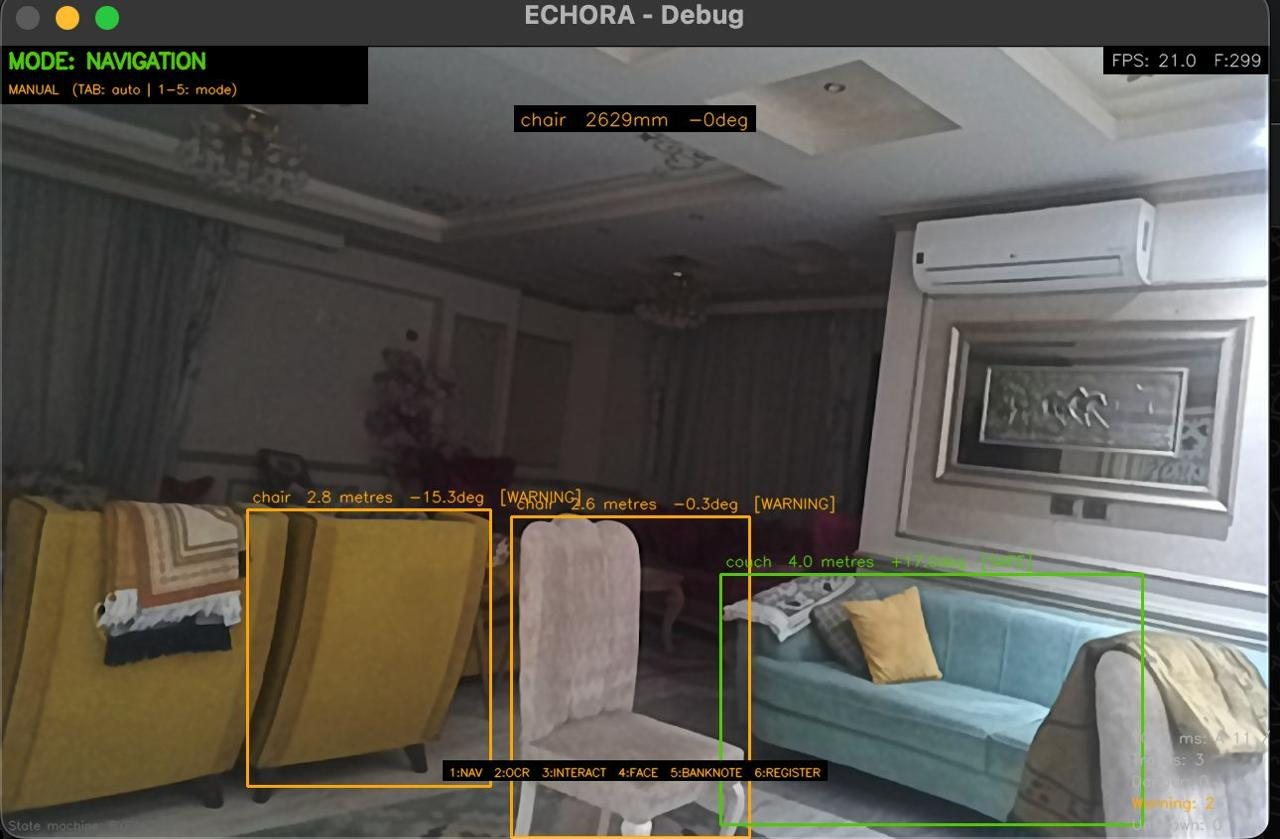
\includegraphics[width=\linewidth,keepaspectratio]{debug_nav_warning.jpg}\\[2pt]
  {\footnotesize (a) Multiple obstacles in the warning zone}
\end{minipage}\hfill
\begin{minipage}[t]{0.49\textwidth}\centering
  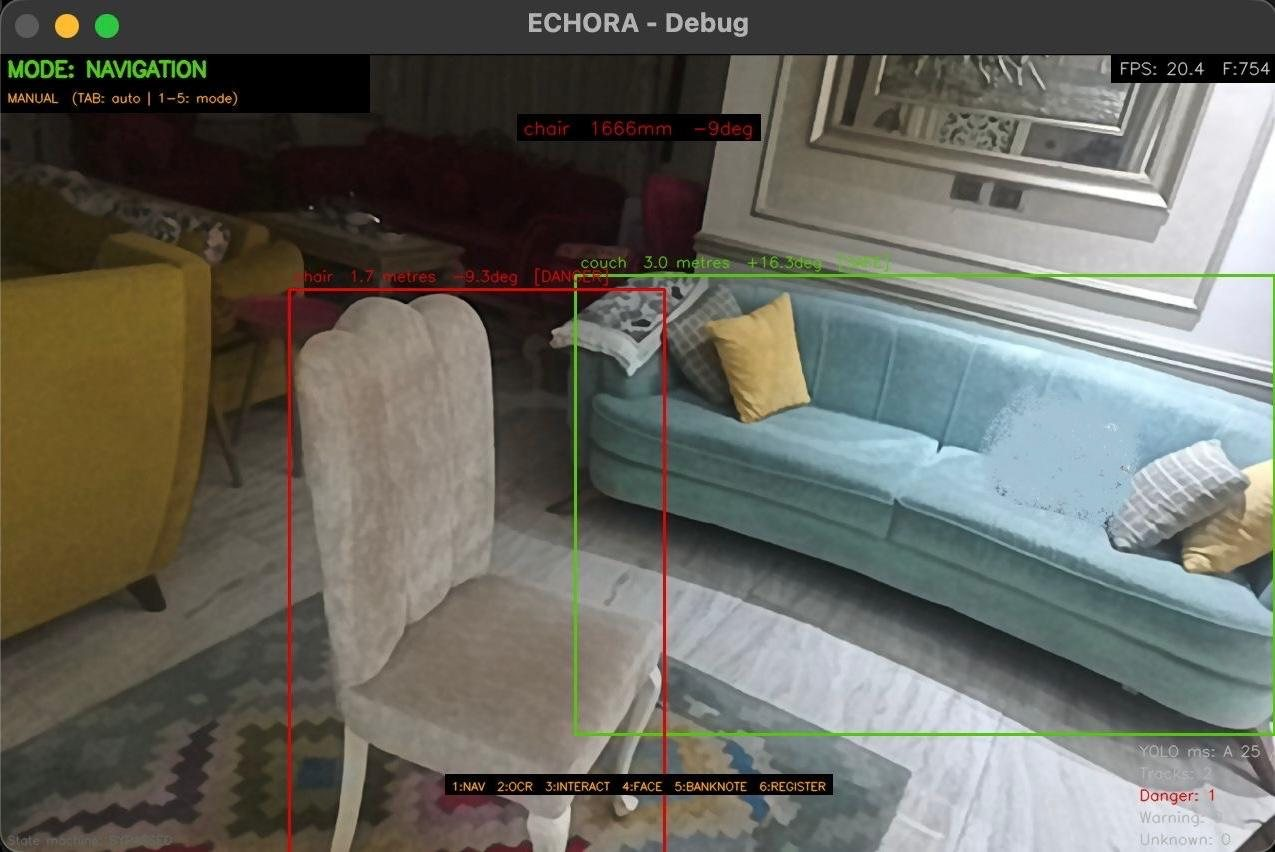
\includegraphics[width=\linewidth,keepaspectratio]{debug_nav_danger.jpg}\\[2pt]
  {\footnotesize (b) Danger obstacle (red) vs.\ safe couch (green)}
\end{minipage}
\caption{Live end-to-end operation in navigation mode, from the real-time debug window. Each detection shows its class, distance, and bearing and is coloured by proximity zone; the display reports the active mode, frame rate ($\sim$20~FPS), and per-zone object counts.}
\label{fig:debug}
\source{Teamwork}
\end{figure}

\section{Discussion of Results}

Taken together, the results support the project's central claim: a unified, real-time, privacy-preserving assistive system can be built on ordinary hardware. The banknote model is genuinely strong; the accessibility model is usable but limited by one badly imbalanced class; the software passes its automated tests; and the full system runs in real time while respecting the safety-first rule.

Two honest limitations frame these results. First, the accuracy figures are the models' own test-set scores, not a measure of how helpful the system feels to a real BLV user; that requires user studies, which were beyond this prototype's scope. Second, the real-time runs confirm correct behaviour and frame rate, but a full account of latency, recognition accuracy in the wild, and safety-alert response time would need a dedicated hardware acceptance test. These are exactly the next steps set out in the following chapter.

\chapter{Conclusions and Recommendations}
\label{ch:conclusion}

\section{Conclusions}

This project set out to design, build, and evaluate Echora: a wearable, AI-powered sensory-substitution system that gives blind and low-vision users a richer, real-time sense of their surroundings through audio and touch, while keeping all processing local for privacy and speed. On the whole, the project met that aim. A complete prototype was produced, covering both the software pipeline and the physical wearable hardware, and it was shown to work as an integrated, real-time system rather than a loose collection of separate features.

It is worth judging the outcome honestly against the objectives set out in Chapter~\ref{ch:intro}.

\begin{itemize}
    \item \textbf{Build the wearable sensing and feedback hardware.} Achieved. A 3D-printed, hand-finished headset carries the depth camera and power, and a custom-designed circuit board drives a twenty-motor wrist array from only three microcontroller pins with cleanly separated power rails. The one caveat is that the camera is currently wired to the computer rather than wireless.
    \item \textbf{Provide continuous obstacle awareness with clear zones.} Achieved. Navigation detects and tracks objects, reads their distance from the depth map, sorts them into danger, warning, and safe zones, and communicates direction through panned audio and vibration.
    \item \textbf{Add practical everyday functions.} Achieved. Text reading, face recognition, banknote identification, and hand guidance were all implemented and tested.
    \item \textbf{Unify everything under a safety-first controller.} Achieved, and this is arguably the project's strongest result. The state machine switches modes automatically and always returns to navigation when danger appears, a rule confirmed in every test scenario.
    \item \textbf{Run in real time on ordinary hardware without the cloud.} Achieved. The full pipeline sustained roughly 20 frames per second locally, with heavy work pushed onto background threads.
    \item \textbf{Evaluate models and system against clear criteria.} Achieved. The banknote detector reached mAP@0.5 of 0.991 and the accessibility detector 0.726; all 22 automated tests passed; and the end-to-end scenarios behaved correctly.
\end{itemize}

The project therefore validates its central idea. It shows that modern computers are capable of supporting advanced assistive technology without specialised infrastructure, and that combining several functions under one safety-aware controller is both feasible and valuable. The clearest technical successes were the custom banknote model and the reliable danger override; the clearest technical weakness was the imbalanced ``updown'' class in the accessibility model, which is a data problem rather than a design flaw.

\section{Critical Reflection}

Several honest limitations should temper these conclusions. The accuracy figures are the models' own test-set scores; they measure detection quality, not how genuinely helpful the system feels to a BLV user in daily life. No formal user study was carried out, so the most important question, namely whether Echora actually makes everyday tasks easier and safer, remains to be answered properly. The banknote test set, though unseen in training, came from a setting similar to the training data, so real-world robustness may be lower. The prototype is also tethered by a wired camera and stores face data without encryption at rest, both of which matter for a device that is meant to be worn all day and to handle biometric information.

The team also learned a good deal about process. Treating real-time performance and safety as hard requirements from the start, rather than optimising them at the end, shaped the architecture in ways that paid off, particularly the decision to run heavy operations on background threads and to debounce every mode switch. Building the hardware in parallel with the software surfaced integration issues early. If the project were repeated, more time would be reserved up front for gathering balanced datasets, since the one weak model was let down by data rather than by method.

\section{Recommendations for Future Work}

The prototype validates the core pipeline, and a clear set of next steps would move it toward a genuinely deployable aid:

\begin{itemize}
    \item \textbf{Wireless wearable link.} Move sensing fully onto the head unit and stream colour and depth to the computer over a wireless link, removing the physical tether while preserving the real-time latency targets.
    \item \textbf{Encrypt biometric data at rest.} Add strong (for example, AES-256) encryption for all stored face embeddings and sensitive data, fully delivering the privacy-by-design goal, together with a clear consent workflow for enabling face recognition and for reviewing or deleting stored identities.
    \item \textbf{Balance and expand the accessibility dataset.} Collect many more examples of the under-represented control classes (especially ``updown''), rebalance the dataset, and retrain to close the one clear accuracy gap.
    \item \textbf{Interpret signs, not just text.} Extend the reading pipeline to classify and announce the \emph{meaning} of traffic, warning, and informational signs, rather than only reading their literal text.
    \item \textbf{Run formal user studies.} Evaluate Echora with BLV participants in realistic tasks, measuring not only accuracy but learnability, comfort, trust, and real reductions in collisions and interaction errors.
    \item \textbf{Full hardware acceptance testing.} Carry out a dedicated test on the complete wearable that captures frame rate, end-to-end latency, in-the-wild recognition accuracy, and safety-alert response time under varied conditions.
\end{itemize}

\section{Closing Remarks}

Echora demonstrates a practical, scalable, and privacy-preserving approach to assistive technology. By fusing depth and vision, delivering information through both hearing and touch, and uniting five everyday functions under a single safety-first controller, it moves beyond the fragmented, single-task tools that dominate the market today. The prototype is not a finished product, and this report has been careful to say where it falls short. But it does provide a solid, working foundation and a clear road map for building assistive technology that could meaningfully increase the independence, safety, and confidence of blind and low-vision people.


% ============================================================
%  END MATTER
% ============================================================
\clearpage
\chapter*{References}
\addcontentsline{toc}{chapter}{References}

\begingroup
\setlength{\parindent}{0pt}
\setlength{\parskip}{0pt}
\raggedright

\refent{Abdelrahman, Y. (no date) \emph{Egyptian banknote YOLOv8} [Dataset]. Available at: \url{https://app.roboflow.com/youssef-abdelrahman/egyptian_-banknote_yolov8/train} (Accessed: 11 July 2026).}

\refent{Bhat, N. M. (2017) \emph{pyttsx3} [Computer program]. Available at: \url{https://github.com/nateshmbhat/pyttsx3} (Accessed: 11 July 2026).}

\refent{Chebat, D.-R., Schneider, F. C., Kupers, R. and Ptito, M. (2011) `Navigation with a sensory substitution device in congenitally blind individuals', \emph{NeuroReport}, 22(7), pp.~342--347.}

\refent{Chen, Y., Shen, J. and Sawada, H. (2023) `A wearable assistive system for the visually impaired using object detection, distance measurement and tactile presentation', \emph{Intelligent Robotics}, 3(3), pp.~420--435.}

\refent{DeepInsight (2017) \emph{InsightFace: RetinaFace detection and ArcFace recognition} [Computer program]. Available at: \url{https://github.com/deepinsight/insightface} (Accessed: 11 July 2026).}

\refent{Envision (2026a) \emph{Envision Glasses}. Available at: \url{https://www.letsenvision.com/glasses/home} (Accessed: 11 July 2026).}

\refent{Envision (2026b) \emph{OCR-based assistance and practical constraints for smart glasses}. Available at: \url{https://support.letsenvision.com/hc/en-us/article_attachments/34626027065361} (Accessed: 11 July 2026).}

\refent{Google (2019) \emph{MediaPipe} [Computer program]. Available at: \url{https://github.com/google-ai-edge/mediapipe} (Accessed: 11 July 2026).}

\refent{Google (2024) \emph{Gemma open models}. Available at: \url{https://ai.google.dev/gemma} (Accessed: 11 July 2026).}

\refent{Lin, Y., Wang, K., Yi, W. and Lian, S. (2019) `Deep learning based wearable assistive system for visually impaired people', \emph{Proceedings of the IEEE/CVF International Conference on Computer Vision (ICCV) Workshops}. Seoul, Republic of Korea, 27--28 October. Piscataway, NJ: IEEE.}

\refent{Luxonis (2019) \emph{DepthAI documentation and the OAK-D depth camera}. Available at: \url{https://docs.luxonis.com/} (Accessed: 11 July 2026).}

\refent{Neugebauer, A., Rifai, K., Getzlaff, M. and Wahl, S. (2020) `Navigation aid for blind persons by visual-to-auditory sensory substitution: a pilot study', \emph{PLoS ONE}, 15(8), e0237344. Available at: \url{https://doi.org/10.1371/journal.pone.0237344} (Accessed: 11 July 2026).}

\refent{Ollama (2023) \emph{Ollama} [Computer program]. Available at: \url{https://ollama.com/} (Accessed: 11 July 2026).}

\refent{OpenCV (2000) \emph{OpenCV} [Computer program]. Available at: \url{https://opencv.org/} (Accessed: 11 July 2026).}

\refent{OrCam Technologies (2023) \emph{OrCam MyEye}. Available at: \url{https://www.orcam.com/en-ie/orcam-myeye} (Accessed: 11 July 2026).}

\refent{PaddlePaddle (2020) \emph{PaddleOCR (PP-OCR)} [Computer program]. Available at: \url{https://github.com/PaddlePaddle/PaddleOCR} (Accessed: 11 July 2026).}

\refent{Pygame (2000) \emph{pygame} [Computer program]. Available at: \url{https://www.pygame.org/} (Accessed: 11 July 2026).}

\refent{PyTorch (2016) \emph{PyTorch} [Computer program]. Available at: \url{https://pytorch.org/} (Accessed: 11 July 2026).}

\refent{RobikScube (2021) \emph{TextOCR: text extraction from images dataset} [Dataset]. Available at: \url{https://www.kaggle.com/datasets/robikscube/textocr-text-extraction-from-images-dataset} (Accessed: 11 July 2026).}

\refent{Schwartz, B. S., King, S. and Bell, T. (2024) `EchoSee: an assistive mobile application for real-time 3D environment reconstruction and sonification supporting enhanced navigation for people with vision impairments', \emph{Bioengineering}, 11(8), 831. Available at: \url{https://doi.org/10.3390/bioengineering11080831} (Accessed: 11 July 2026).}

\refent{Seleste (2023) \emph{Seleste glasses}. Available at: \url{https://www.seleste.co/} (Accessed: 11 July 2026).}

\refent{Shull, P. B. and Damian, D. D. (2015) `Haptic wearables as sensory replacement, sensory augmentation and trainer: a review', \emph{Journal of NeuroEngineering and Rehabilitation}, 12, 59. Available at: \url{https://doi.org/10.1186/s12984-015-0055-z} (Accessed: 11 July 2026).}

\refent{SQLAlchemy (2006) \emph{SQLAlchemy} [Computer program]. Available at: \url{https://www.sqlalchemy.org/} (Accessed: 11 July 2026).}

\refent{St\"uckler, J., Waldvogel, B., Schulz, H. and Behnke, S. (2015) `Dense real-time mapping of object-class semantics from RGB-D video', \emph{Journal of Real-Time Image Processing}, 10(4), pp.~599--609. Available at: \url{https://doi.org/10.1007/s11554-013-0379-5} (Accessed: 11 July 2026).}

\refent{Sun Moon University (2022) \emph{Elevator button recognition} [Dataset]. Available at: \url{https://universe.roboflow.com/sun-moon-university/elevator-button-recognition} (Accessed: 11 July 2026).}

\refent{Sunu (2018) \emph{Sunu Band mobility aid} [User manual]. Available at: \url{https://device.report/manual/1594812} (Accessed: 11 July 2026).}

\refent{Teng, S.-Y., Kim, G. S.-H., Liu, X. and Lopes, P. (2025) `Seeing with the hands: a sensory substitution that supports manual interactions', \emph{Proceedings of the 2025 CHI Conference on Human Factors in Computing Systems}. New York: ACM. Available at: \url{https://doi.org/10.1145/3706598.3713419} (Accessed: 11 July 2026).}

\refent{UAEU (2022) \emph{Door and handles detection} [Dataset]. Available at: \url{https://universe.roboflow.com/uaeu/door-and-handles-detection} (Accessed: 11 July 2026).}

\refent{Ultralytics (2023) \emph{Track mode with ByteTrack: Ultralytics YOLO documentation}. Available at: \url{https://docs.ultralytics.com/modes/track/} (Accessed: 11 July 2026).}

\refent{WeWALK (2026) \emph{WeWALK smart cane}. Available at: \url{https://wewalk.io/} (Accessed: 11 July 2026).}

\endgroup


\appendix
\chapter{Appendices}
\addcontentsline{toc}{chapter}{Appendices}

\section*{Appendix A: The Five Perception Modes in Operation}
\addcontentsline{toc}{section}{Appendix A: The Five Perception Modes in Operation}

The screenshots below show Echora's five modes running on real inputs: navigation with proximity-zoned obstacles, text reading, face recognition, banknote identification, and hand-guidance interaction.

\begin{figure}[H]
\centering
\begin{minipage}[t]{0.31\textwidth}\centering
  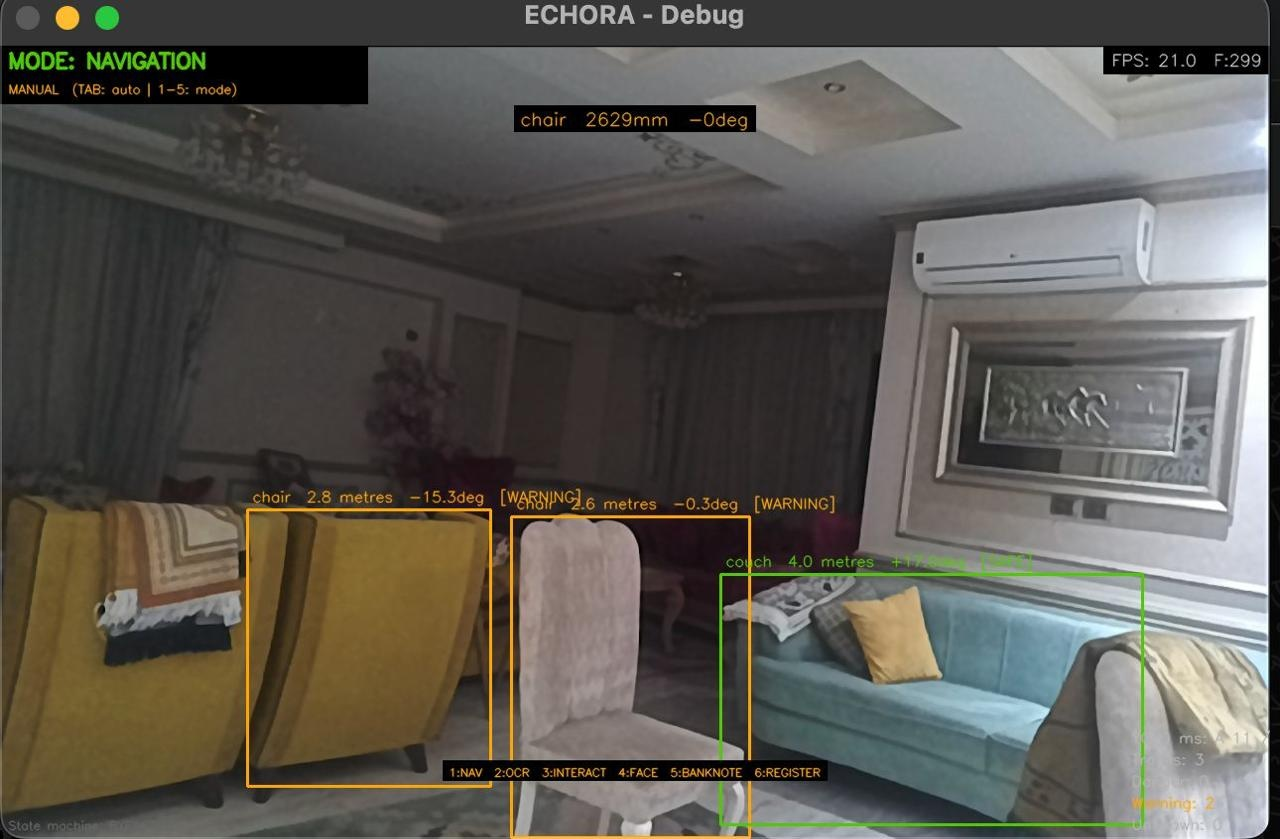
\includegraphics[width=\linewidth,height=3.4cm,keepaspectratio]{mode_navigation.jpg}\\[2pt]{\footnotesize (a) Navigation}
\end{minipage}\hfill
\begin{minipage}[t]{0.31\textwidth}\centering
  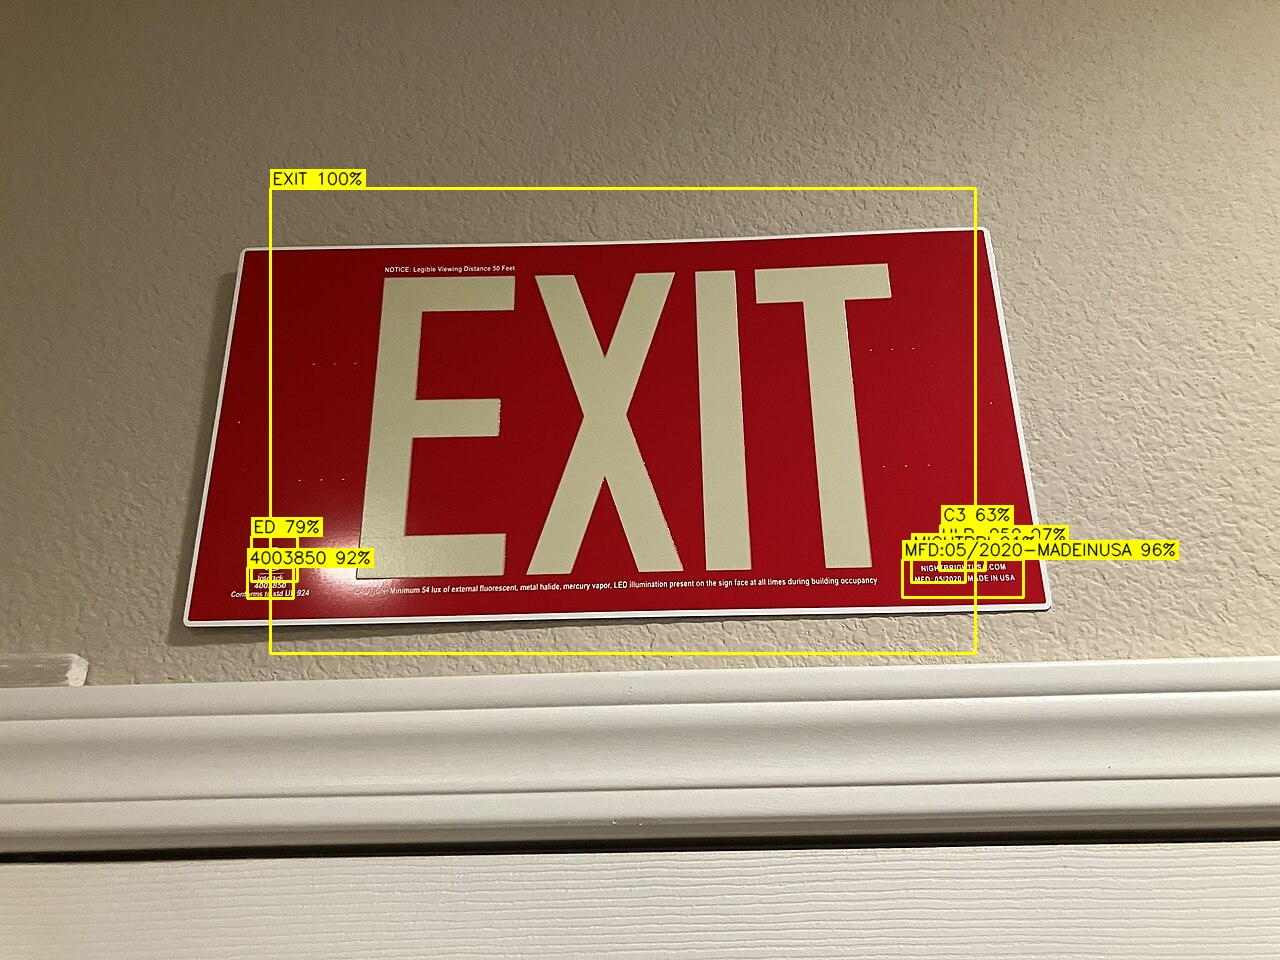
\includegraphics[width=\linewidth,height=3.4cm,keepaspectratio]{mode_ocr.jpg}\\[2pt]{\footnotesize (b) Text reading (OCR)}
\end{minipage}\hfill
\begin{minipage}[t]{0.31\textwidth}\centering
  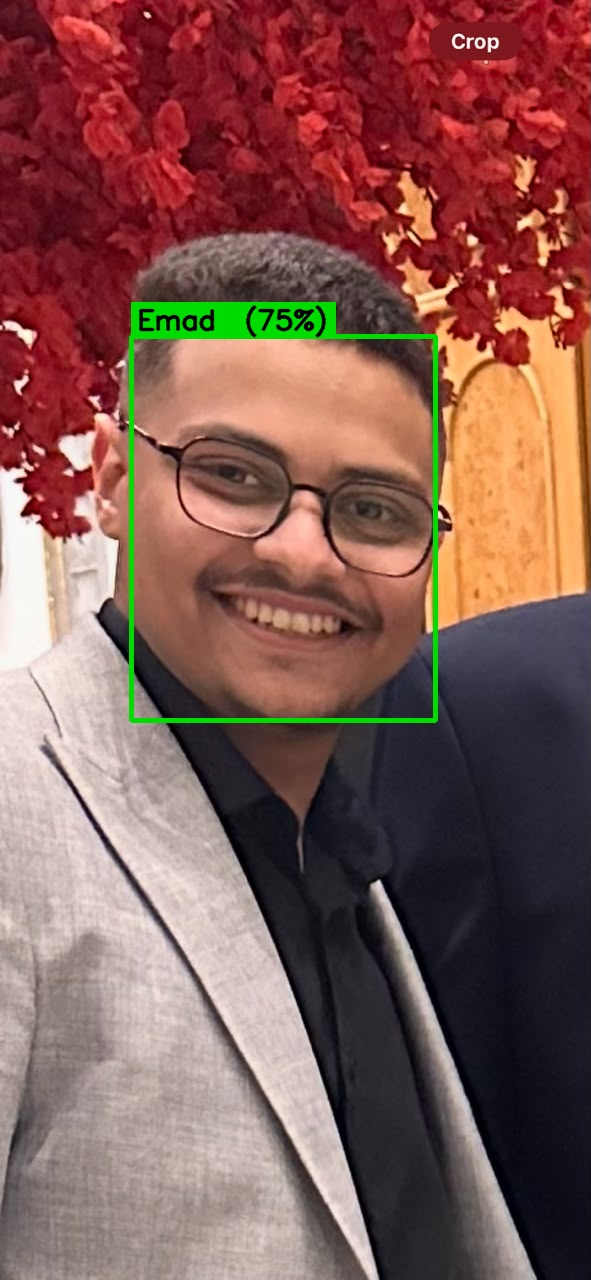
\includegraphics[width=\linewidth,height=3.4cm,keepaspectratio]{mode_face.jpg}\\[2pt]{\footnotesize (c) Face recognition}
\end{minipage}
\\[6pt]
\begin{minipage}[t]{0.31\textwidth}\centering
  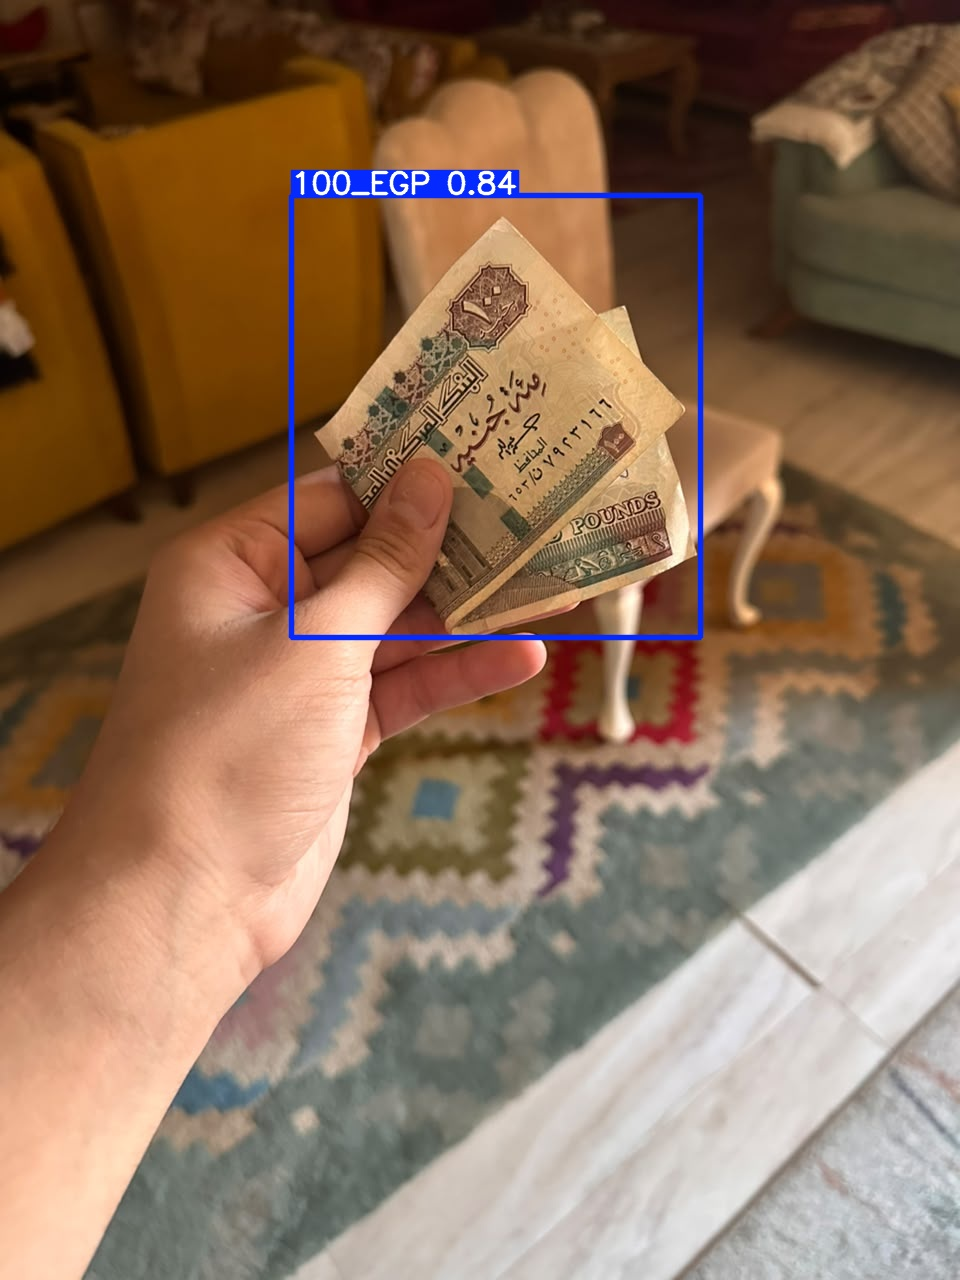
\includegraphics[width=\linewidth,height=3.4cm,keepaspectratio]{mode_banknote.jpg}\\[2pt]{\footnotesize (d) Banknote identification}
\end{minipage}\hfill
\begin{minipage}[t]{0.31\textwidth}\centering
  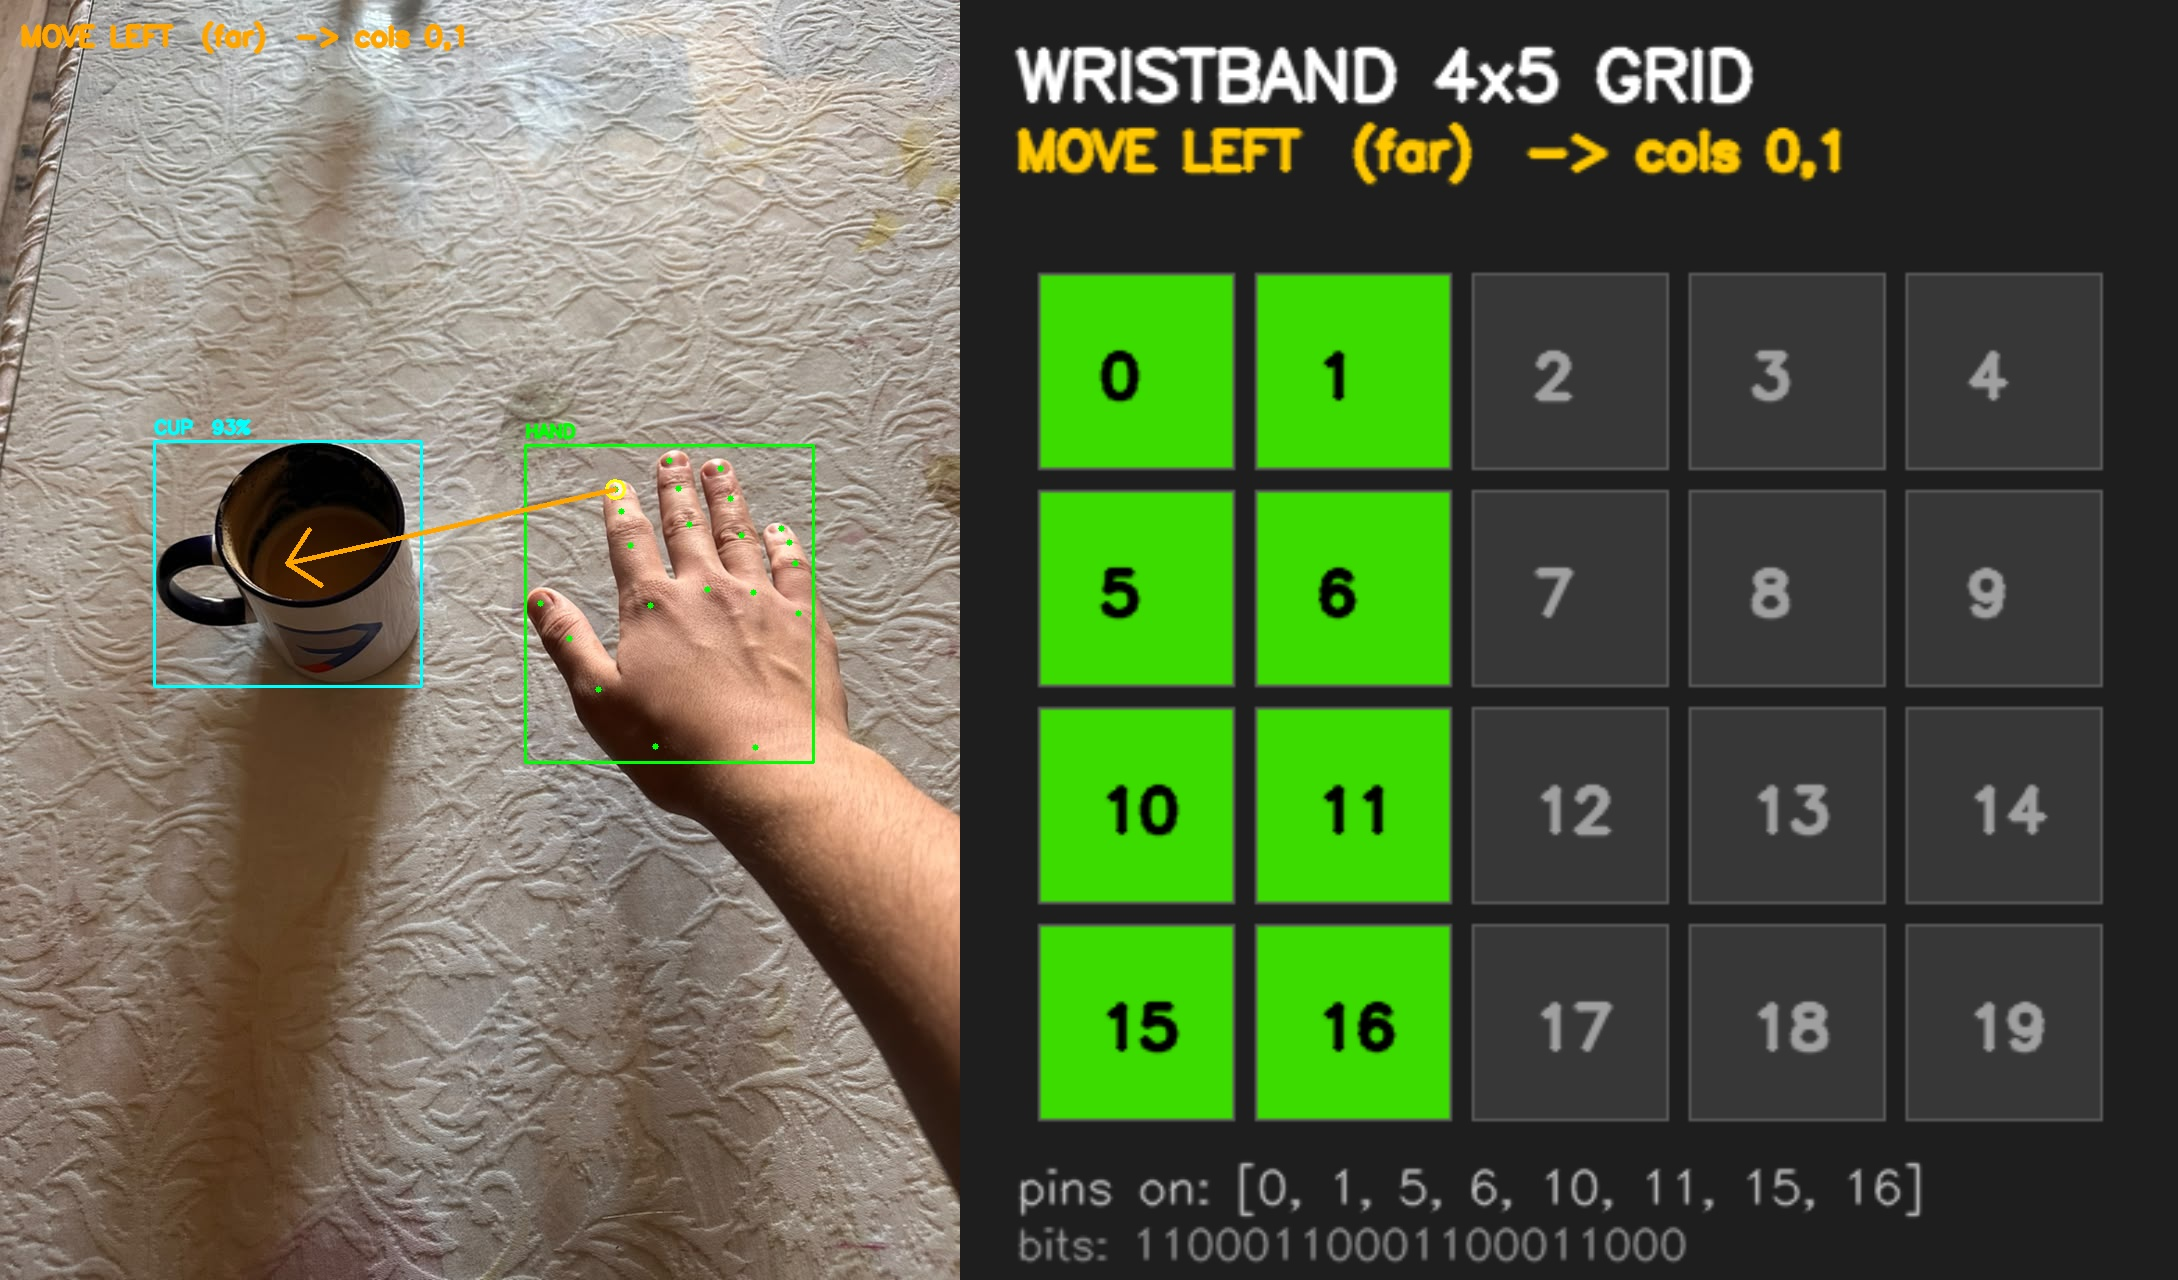
\includegraphics[width=\linewidth,height=3.4cm,keepaspectratio]{mode_interaction.jpg}\\[2pt]{\footnotesize (e) Hand guidance}
\end{minipage}\hfill
\begin{minipage}[t]{0.31\textwidth}\centering
  ~
\end{minipage}
\caption{Echora's five perception modes running on real inputs.}
\label{fig:modes}
\source{Teamwork}
\end{figure}

\section*{Appendix B: Hardware Build Highlights}
\addcontentsline{toc}{section}{Appendix B: Hardware Build Highlights}

The prototype was built by hand. Figure~\ref{fig:build} shows the finished 3D-printed headset and the custom haptic module that drives the wrist array of vibration motors.

\begin{figure}[H]
\centering
\begin{minipage}[b]{0.48\textwidth}\centering
  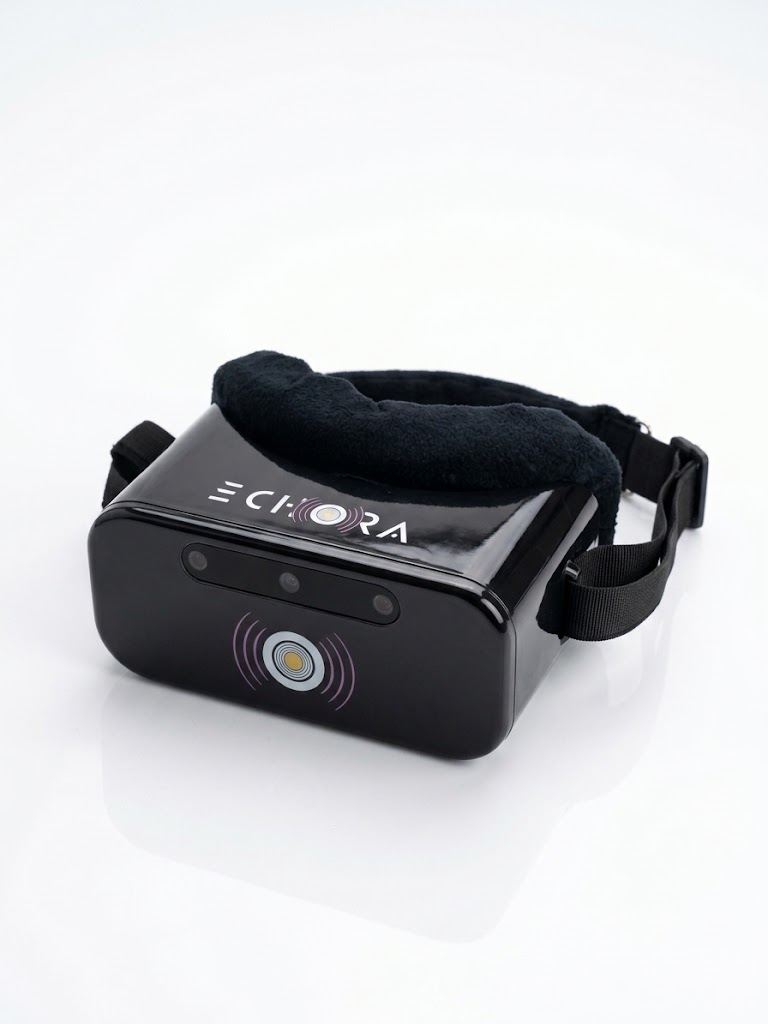
\includegraphics[width=\linewidth,height=5.2cm,keepaspectratio]{build_glasses.jpeg}\\[2pt]{\footnotesize (a) Finished headset}
\end{minipage}\hfill
\begin{minipage}[b]{0.48\textwidth}\centering
  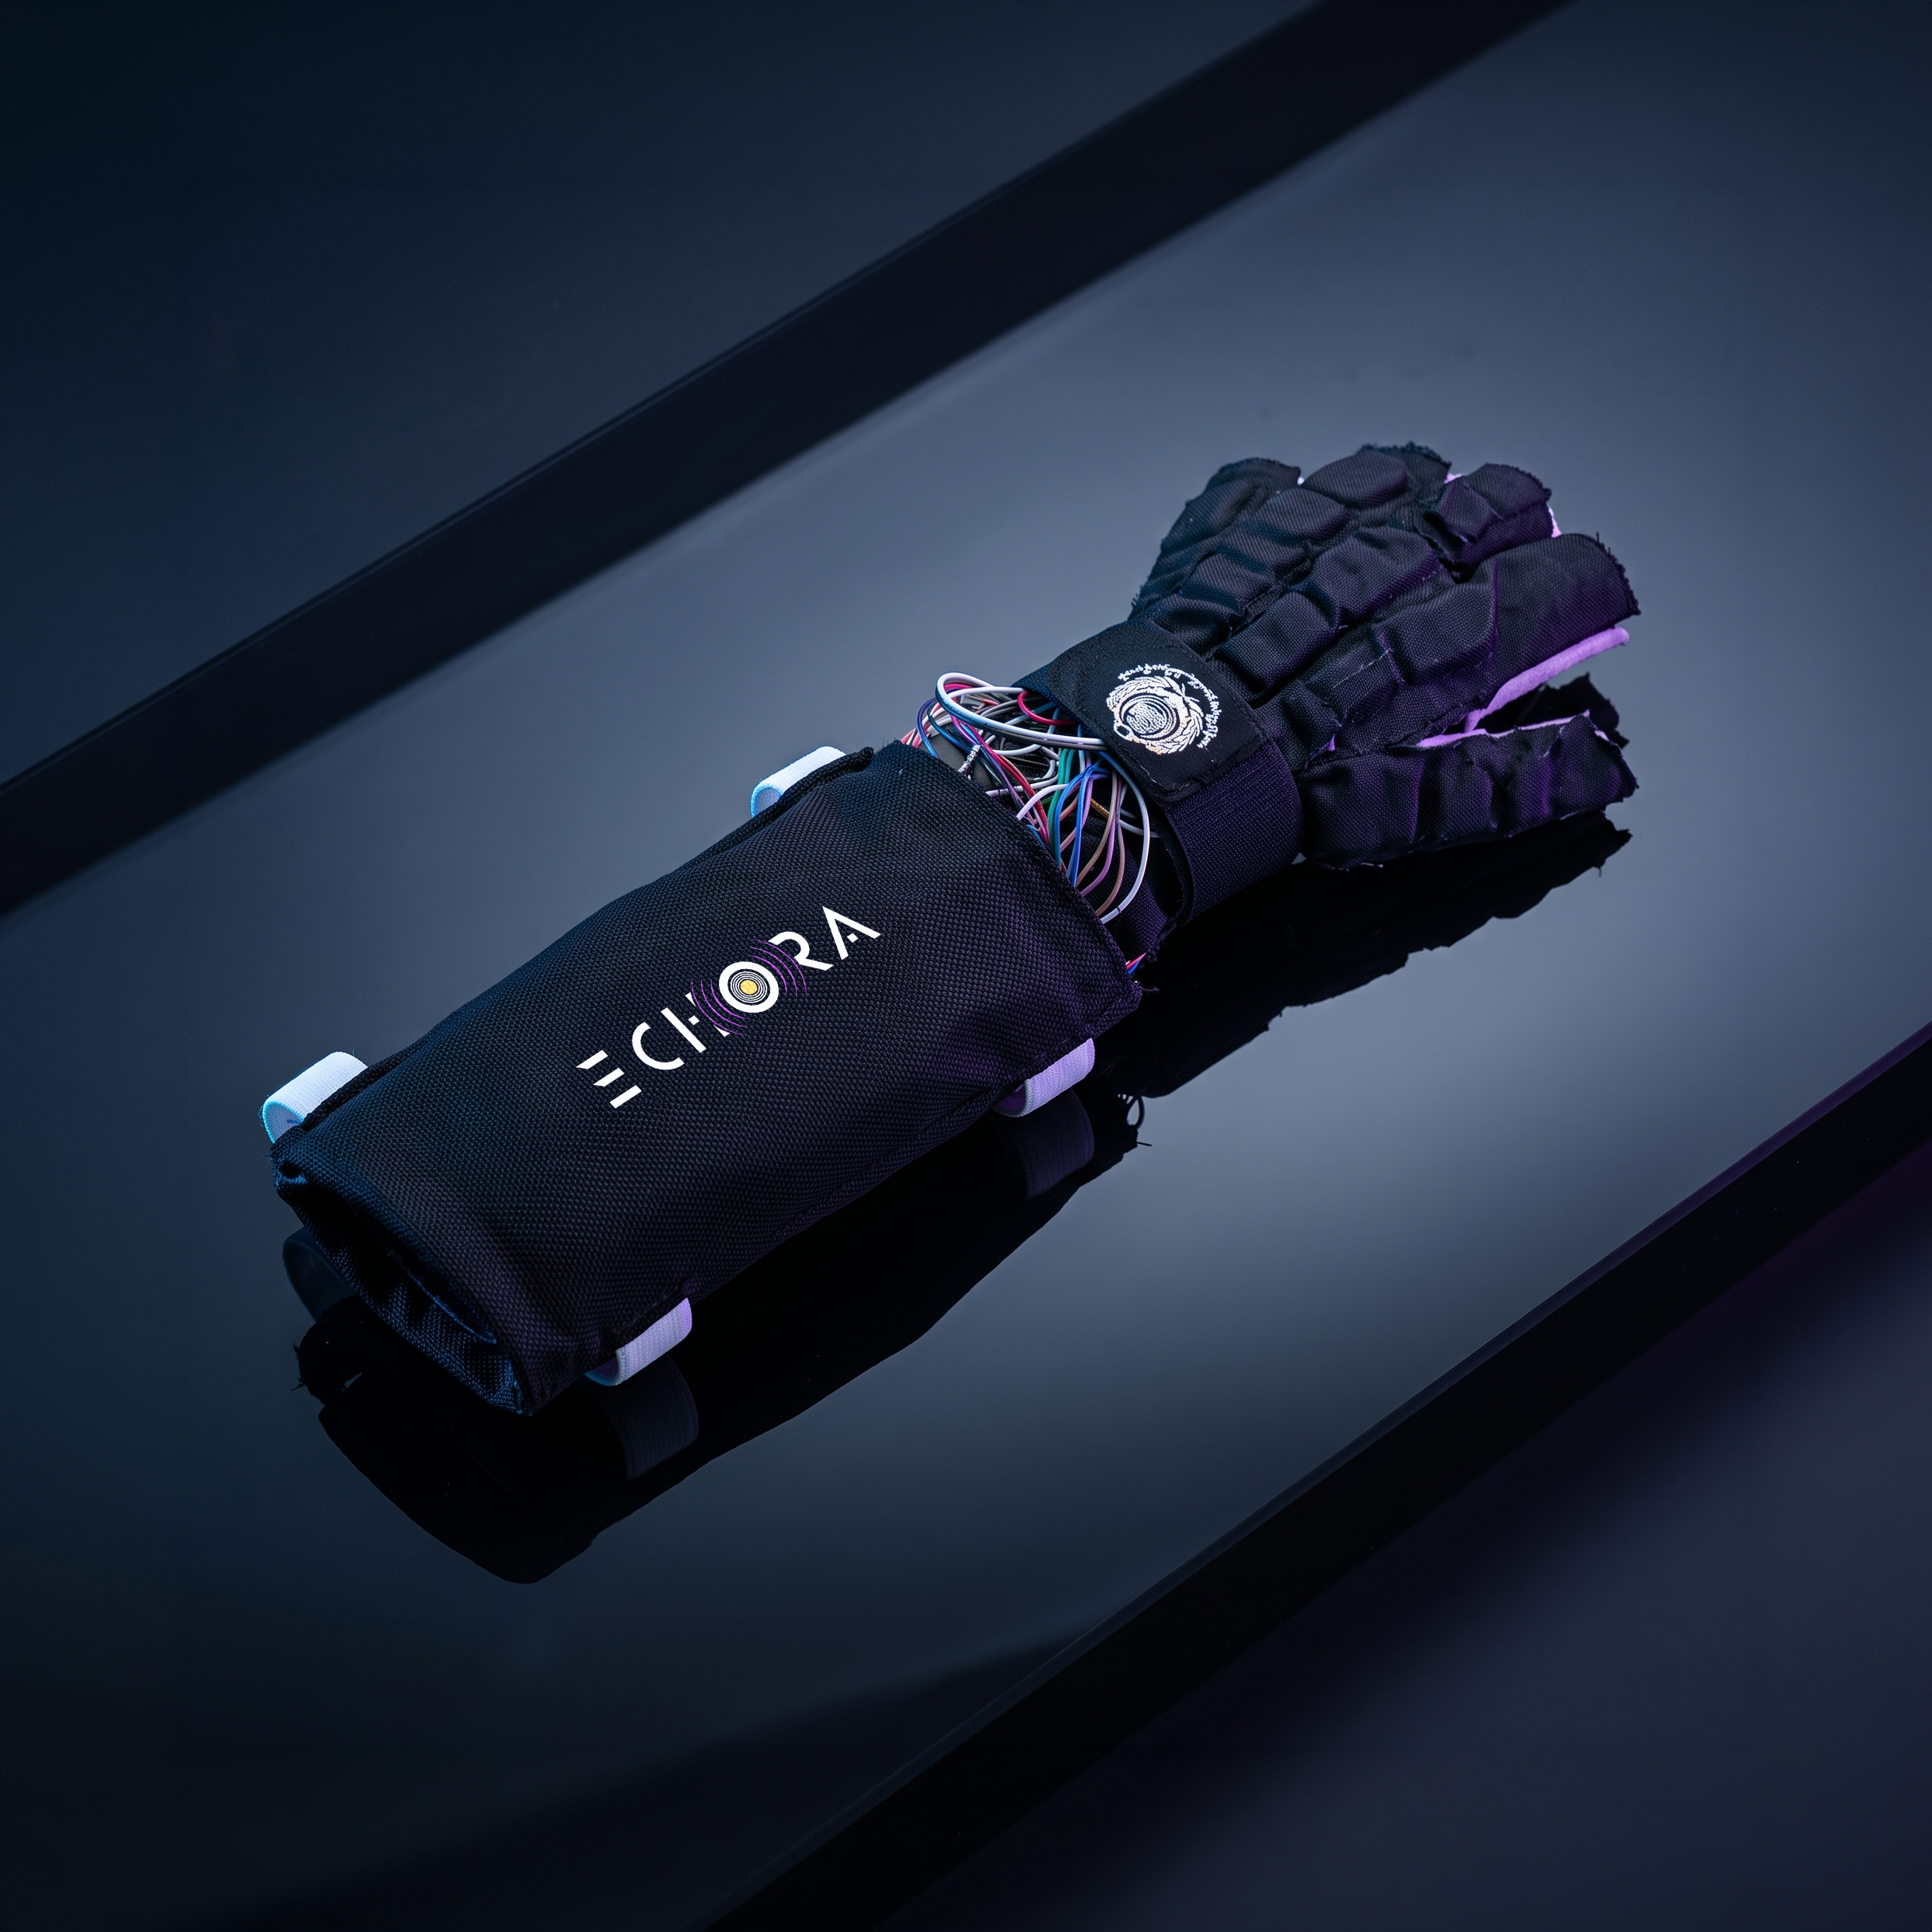
\includegraphics[width=\linewidth,height=5.2cm,keepaspectratio]{build_haptic.png}\\[2pt]{\footnotesize (b) Custom haptic module}
\end{minipage}
\caption{Highlights of the physical prototype build.}
\label{fig:build}
\source{Teamwork}
\end{figure}

\section*{Appendix C: Banknote Model Precision--Recall Curve}
\addcontentsline{toc}{section}{Appendix C: Banknote Model Precision--Recall Curve}

\begin{figure}[H]
\centering
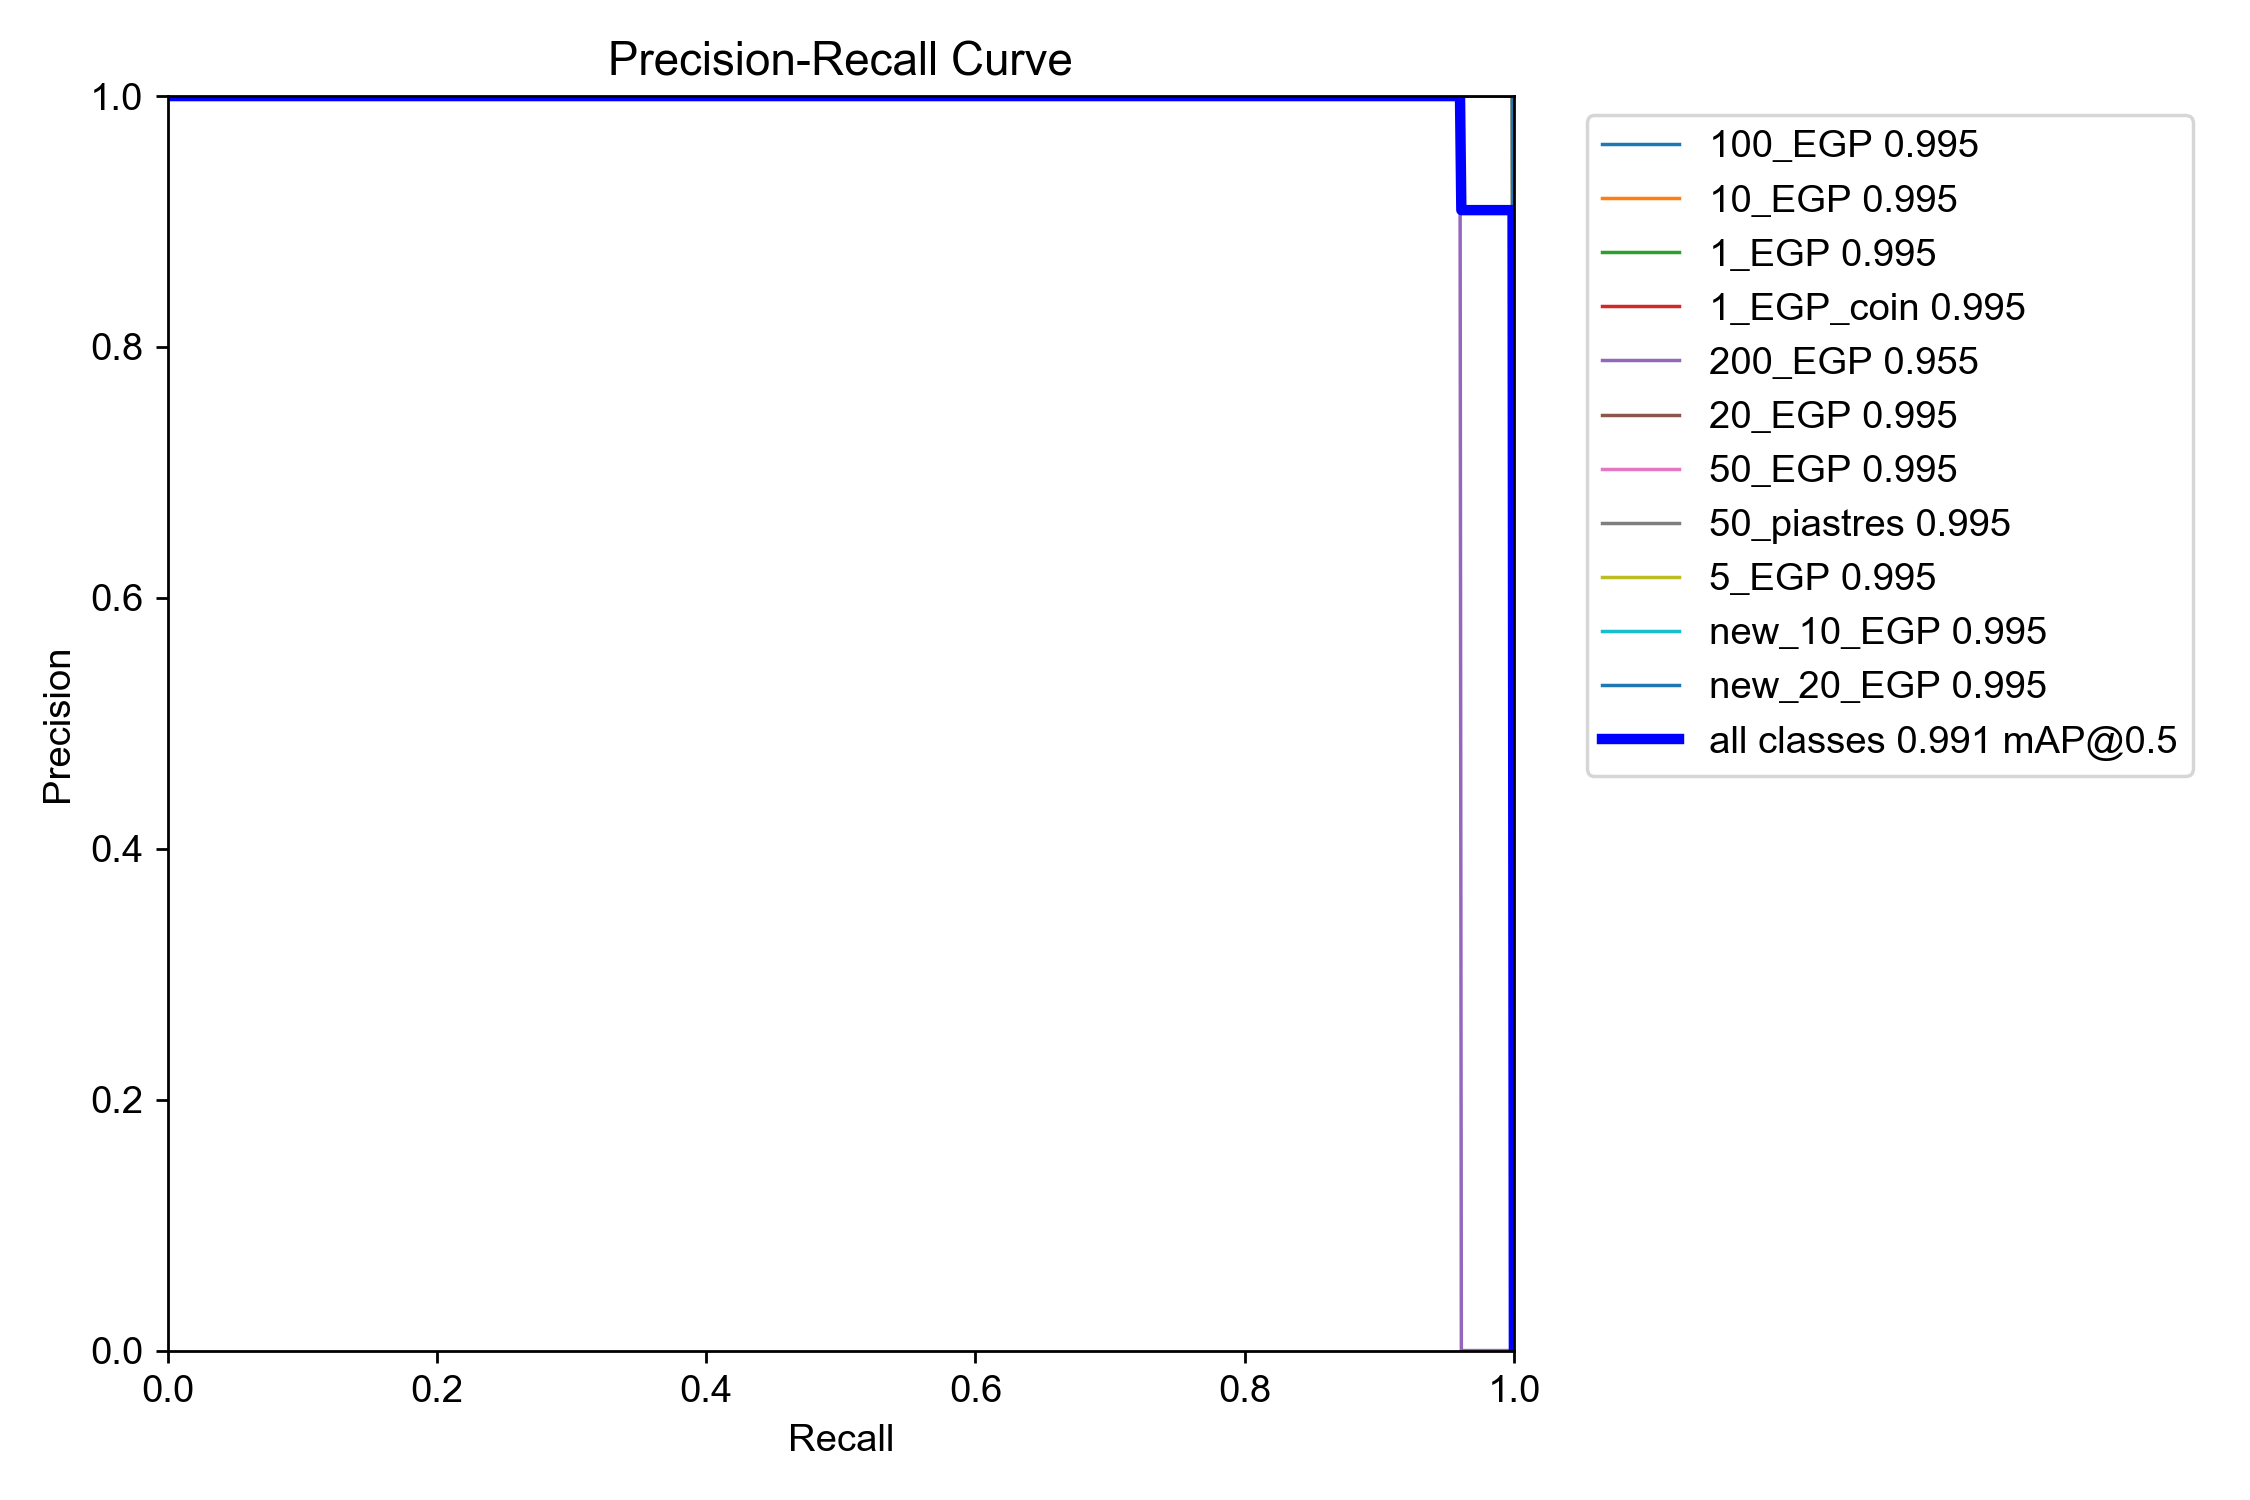
\includegraphics[width=0.72\textwidth,keepaspectratio]{banknote_pr.png}
\caption{Precision--recall curve for the custom Egyptian banknote detector across all eleven denomination classes.}
\label{fig:bank_pr}
\source{Teamwork}
\end{figure}

\section*{Appendix D: Record of Generative AI Use}
\addcontentsline{toc}{section}{Appendix D: Record of Generative AI Use}

This appendix records how generative AI was used in the preparation of this
report, as required by the module guide. The declaration in the preliminary
pages should be read together with this record.

\textbf{Tool used.} A general-purpose generative AI writing assistant, accessed
through its standard web interface.

\textbf{What it was used for.} The tool was used only after we had written a
complete first draft of each chapter ourselves. Its use was limited to language
and presentation:

\begin{itemize}
  \item checking spelling and correcting typing errors;
  \item correcting grammar, punctuation, and sentence structure;
  \item improving the clarity and flow of paragraphs we had already written, so
        that the writing reads in a more formal and professional academic style;
  \item checking that the report followed the required format and structure,
        including consistent headings, captions, and the ordering of sections.
\end{itemize}

\textbf{Typical way it was used.} We pasted a paragraph or section of our own
draft into the tool and asked it to correct the grammar and improve the clarity
without changing the meaning. We then compared its version with our own,
accepted only the changes we agreed with, and rewrote anything that did not
match what we meant. The final wording in this report was chosen by us.

\textbf{What it was not used for.} The tool was not used to generate the ideas,
technical content, system design, code, experimental results, analysis, or
conclusions presented in this report. It was not used to find, suggest, or
produce any reference. Every source in the reference list was located, read, and
checked by the team, and every result reported was produced by running our own
evaluation scripts on our own trained models.

\textbf{Verification.} We are aware that AI-generated text can contain errors,
invented references, or bias. For this reason every sentence that the tool
helped to reword was checked by us against the original draft and against the
underlying technical work, to confirm that the meaning was unchanged and
factually correct.


\end{document}
